% Isaac Dunn Part II Computer Science Dissertation
\documentclass[12pt,a4paper,twoside,openany]{report}
\usepackage[pdfborder={0 0 0}]{hyperref}    % turns references into hyperlinks
\usepackage[margin=25mm]{geometry}  % adjusts page layout
\usepackage[T1]{fontenc}
\usepackage{mathpazo}  % style
\usepackage{graphicx}  % allows inclusion of PDF, PNG and JPG images
\graphicspath{ {./figs/} }
\DeclareGraphicsExtensions{.pdf,.png,.jpg}
\usepackage{verbatim}
\usepackage{docmute}   % only needed to allow inclusion of proposal.tex
\usepackage{amsmath}
\usepackage{amsfonts}
\usepackage{algorithm}
\usepackage[noend]{algpseudocode}
\usepackage{enumitem}
\usepackage{color}
\usepackage{listings}
\usepackage{subcaption}
\usepackage[labelfont=bf]{caption}
\usepackage[sort,nocompress]{cite} % sort multiple citations, but don't group
\usepackage{afterpage} % for adding blank page

\definecolor{dkgreen}{rgb}{0,0.6,0}
\definecolor{grey}{rgb}{0.5,0.5,0.5}
\definecolor{mauve}{rgb}{0.58,0,0.82}
\lstset{ % style of code listings
	frame=tb,
	language=ML,
	aboveskip=3mm,
	belowskip=3mm,
	showstringspaces=false,
	columns=flexible,
	basicstyle={\small\ttfamily},
	numbers=none,
	numberstyle=\tiny\color{grey},
%	keywordstyle=\color{blue},
%	commentstyle=\color{dkgreen},
%	stringstyle=\color{mauve},
	breaklines=true,
	breakatwhitespace=true,
	tabsize=4
	}


\raggedbottom                           % try to avoid widows and orphans
\sloppy
\clubpenalty1000%
\widowpenalty1000%

\renewcommand{\baselinestretch}{1.1}    % adjust line spacing to make
                                        % more readable

% "let a = b in" for use in algorithms
\newcommand{\Let}[2]{\State \textbf{let} #1 = #2 \textbf{in}}

% For use in the happens-before relation varient
\newcommand{\longhookrightarrow}
	{\ensuremath{\lhook\joinrel\longrightarrow}}


\newenvironment{understandinglist}
	{\begin{itemize} \itemsep 0em}{\end{itemize}}

\newenvironment{figtile} % for evaluation graphs
{\begin{subfigure}{0.48\textwidth}
		\def\svgwidth{\textwidth}
		\captionsetup{font=footnotesize}
	}
	{\end{subfigure}}

\begin{document}

\bibliographystyle{plain}


%%%%%%%%%%%%%%%%%%%%%%%%%%%%%%%%%%%%%%%%%%%%%%%%%%%%%%%%%%%%%%%%%%%%%%%%
% Title page

\thispagestyle{empty}

\rightline{\LARGE \textbf{Isaac Dunn}}

\vspace*{60mm}
\begin{center}
\Huge
\textbf{Dynamic Partial-Order Reduction for Model Checking} \\[7mm]
Computer Science Tripos -- Part II \\[6mm]
Clare College \\[7mm]
\LARGE May 2016  % today's date
\end{center}

%%%%%%%%%%%%%%%%%%%%%%%%%%%%%%%%%%%%%%%%%%%%%%%%%%%%%%%%%%%%%%%%%%%%%%%%%%%%%%
% Proforma, table of contents and list of figures

\pagestyle{plain}

\chapter*{Proforma}

{\large
\begin{tabular}{ll}
Name:           &  Isaac Dunn                            			 \\
College:        &  Clare College                    				     \\
Project Title:	&  Dynamic Partial-Order Reduction for Model Checking \\
Examination:    &  Computer Science Tripos -- Part II, June 2016      \\
Word Count:     &  11,624\footnotemark[1]					 \\
Originator: &  Isaac Dunn\footnotemark[2] 					 \\
Supervisors:	&  Dr.\@ Jonathan Hayman \& Prof.\@ Glynn Winskel         \\
\end{tabular}
}
\footnotetext[1]{The program \texttt{wc} was run on a plain-text
	file of Chapters 1--5, with diagram text manually removed.}
\stepcounter{footnote}
\footnotetext[2]{With guidance from Dr. Jonathan Hayman.}
\stepcounter{footnote}


\section*{Original Aim of the Project}

The original aim of the project was to implement
a simple model-checking algorithm, and to
understand and implement the dynamic partial-order reduction
model-checking algorithm.

\section*{Work Completed}

The simple and dynamic partial-order reduction
model-checking algorithms
were implemented, successfully verifying
programs written in a concurrent programming language.
Several extensions were
also completed, including implementations of
stateful model checking, sleep sets,
static partial-order reduction,
and visualisation of counter-example
traces. A quantitative comparison of the
performances of the implemented
algorithms was also completed.

\section*{Special Difficulties}

No special difficulties were encountered.
 
\section*{Declaration of Originality}

I, Isaac Dunn of Clare College, being a candidate for Part II of the Computer
Science Tripos, hereby declare
that this dissertation and the work described in it are my own work,
unaided except as may be specified below, and that the dissertation
does not contain material that has already been used to any substantial
extent for a comparable purpose.

\bigskip
\leftline{Signed:}

\bigskip
\leftline{Date:}

\bigskip\bigskip
\section*{Acknowledgements}

I would like to thank my supervisor,
Dr.\@ Jonathan Hayman, for all his help
and guidance this year. I am
also grateful to Prof.\@ Glynn Winskel for
agreeing to nominally supervise me,
in case Dr.\@ Hayman could not continue
for the entire year. Finally, I would
like to express my gratitude to anyone
who has ever taught me anything, without
whom I would know nothing.

\setcounter{tocdepth}{1} % hide subsections
\tableofcontents

%%%%%%%%%%%%%%%%%%%%%%%%%%%%%%%%%%%%%%%%%%%%%%%%%%%%%%%%%%%%%%%%%%%%%%%
% now for the body

\pagestyle{headings}

\chapter{Introduction}
After reading this chapter,
you should understand:
\begin{understandinglist}
	\item what model checking is and why it is useful;
	\item what the state explosion problem is;
	\item how partial-order reduction
	techniques address the state explosion problem; and
	\item the aims of my project.
\end{understandinglist}

\section{Model Checking}
%After reading this section,
%you should understand why formal methods for
%verifying the correctness of software and
%hardware systems are useful, that model
%checking is such a formal method, and
%how model checking works.

There are many reasons for ensuring that
software and hardware systems have as
few defects as possible. Failure of a
safety- or mission-critical system can
have devastating consequences, but even the
presence of bugs in everyday commercial systems has
serious economic implications. In 2002,
software bugs were estimated to cost
the U.S. economy \$59.5 billion per year \cite{tass02}.

Complementary to traditional testing
and peer review, formal verification methods have been
increasingly used
to minimise the number of defects in a
software or hardware system. A formal
method uses automated
mathematical analysis to increase
the confidence that a system meets its
specification, or shows that it does not.

Model checking is a verification method
that arose in the early 1980s,
motivated by the desire to automatically
verify concurrent programs \cite{cla08}.
A model-checking algorithm performs
an exhaustive enumeration of a given
system's behaviour to show that it
satisfies some property, usually
expressed in a temporal logic.

The idea of applying Tarski
fixed-point techniques \cite{tar55}
to automatically check that a
program, expressed as a finite-state
system, meets a specification
expressed in a propositional
temporal logic was independently introduced
by Clarke and Emerson \cite{cla82} and
Queille and Sifakis \cite{que82}. Vardi and
Wolper later devised an algorithm that
performs model checking efficiently
for the other main type of temporal
logic, which treats time in terms
of continuous paths rather than branching
trees \cite{var96}.
Other important
milestones in the history of model
checking include McMillan's
symbolic model checking \cite{mcm93},
which allowed much larger
systems to be verified;
bounded model checking, introduced by
Biere et al.\@ \cite{bie99},
which allowed model checking
to find bugs in systems too large for full
verification; automatic counterexample-guided
abstraction refinement by Clarke et al.\@
\cite{cla00}, which allowed simpler but
in some sense equivalent models
(abstractions) to be easily used; and
various partial-order techniques, discussed
below.

Model checking has been used with considerable
success in practice, for instance in finding
a long-standing flaw in the Needham-Schroeder
security protocol \cite{low96},
integration into the IBM \cite{sch97} and Amazon
\cite{new15}
development processes,
and verification of
software controlling a flood barrier near
Rotterdam \cite{kars96},
a NASA Mars Rover \cite{brat04},
and an ``industrial-size design of an
ultra-modern satellite platform'' \cite{est12}.

\section{The State Explosion Problem}
%After reading this section, you should
%understand what the state explosion problem
%is, and its implications for model checking.

Unlike conventional testing, which notoriously
struggles to expose concurrency bugs,
model checking can verify that concurrent
programs are free of deadlocks, livelocks, or
race conditions that could result in
an error. However, model checking
suffers from what is known as the
\textit{state explosion problem}.

Consider a concurrent system consisting
of $n$ asynchronous processes, each of which
has $k$ instructions to execute before it
terminates. Unfortunately for model checking,
there are
\[N =\frac{(kn)!}{(k!)^n}\]
different interleavings of the instructions
from the different threads.
If each different interleaving
can result in a different final system state,
then each of these must be checked,
meaning that the running time of any model
checker is $N$ in
the worse case.
Figure~\ref{fig:state-explosion} shows
how $N$ grows for $k = 1$.

\begin{figure}
	\centering
	\begin{subfigure}{0.15\textwidth}
		\centering
		\includegraphics*[height=3cm]{explosion1}
	\end{subfigure}
	\quad
	\begin{subfigure}{0.25\textwidth}
		\centering
		\includegraphics*[height=5cm]{explosion2}
	\end{subfigure}
	\quad
	\begin{subfigure}{0.5\textwidth}
		\centering
		\includegraphics*[height=5cm]{explosion3}
	\end{subfigure}
	\begin{subfigure}{\textwidth}
		\centering
		\includegraphics*[width=\textwidth]{explosion4}
	\end{subfigure}
	\caption[Illustration of the state explosion problem.]
		{Diagrams showing the possible interleavings of
			one, two, three and four events.}
	\label{fig:state-explosion}
	
	\includegraphics*[height=11cm]{por}
	\caption[Illustration of partial-order reduction.]
	{If the order of execution of four instructions or
		events makes no difference to the end result, it
		suffices to check only one interleaving.}
	\label{fig:por}
\end{figure}

\section{Partial-Order Reduction}
%After reading this section, you should
%understand how partial-order reduction
%techniques address the state
%explosion problem.

Model checking is still used in practice, thanks
to various techniques that mitigate
the state explosion problem. Partial-order reduction
techniques reduce the number
of interleavings that must be explored
by using the fact that the order
of execution of some instructions makes
no difference to the end result.
Fully exploiting
this idea can very effectively mitigate the
state explosion problem, as shown in
Figure~\ref{fig:por}.

Valmari's stubborn sets \cite{val90},
Peled's ample sets \cite{pel94},
and Godefroid's persistent and sleep sets
\cite{god91} are
instances of partial-order reduction;
incidentally, the
latter two are explored as extensions to
my project.

\section{My Project}
%After reading this section, you should
%understand the idea behind the dynamic
%partial-order reduction algorithm, and
%the nature of my project.

At the 2005 Principles
of Programming Languages (POPL) conference,
Flanagan and Godefroid presented
a paper titled Dynamic Partial-Order Reduction
for Model Checking Software  \cite{flan05},
introducing an algorithm
which uses information gathered dynamically
during its
exploration of a state space
to perform partial-order reduction more
effectively than existing algorithms.
In particular, it initially assumes that
all possible interleavings of
instructions in a concurrent program will
give the same result, and only explores
alternative executions when it discovers
pairs of instructions that might give
different results when executed in a
different order.

The original aim of my project was to
fully implement the dynamic partial-order
reduction (DPOR) algorithm presented in the POPL
paper from scratch, and to evaluate its performance
against a simple model-checker
that performs no partial-order reduction.
These goals were successfully
achieved, and several other model-checking
algorithms and techniques were also
implemented as extensions. This allowed
a fuller evaluation of the performance
of DPOR in comparison to other techniques.

\chapter{Preparation}
\label{cha:prep}
After reading this chapter,
you should understand:
\begin{understandinglist}
	\item the work I undertook before beginning
	the implementation of my project;
	\item the background theory of model checking
	relevant to my project;
	\item the persistent-set
	and sleep-set partial-order reduction techniques; and
	\item the basic operation of the DPOR algorithm.
\end{understandinglist}

\section{Preparatory Work}

\subsection{Research and Understanding}

In order to fully implement the
POPL paper introducing dynamic partial-order
reduction \cite{flan05}, I first needed
to find and read academic papers
covering the relevant
background theory, and then
read and understand the paper itself.
This exploration
of a new area of computer science was the
main preparation that was necessary
before I could begin implementing
my project. The remaining sections
of this chapter explain the core
of this material that is essential
to understand my project.

\subsection{Requirements Analysis}
Having understood the necessary theory,
I refined the goals of my project to
make them as concrete as possible.
I decided on exactly what the
model-checking algorithms would
take as their inputs and give
as their outputs, and
explicitly set out the need
to implement
a programming language
to express concurrent programs
for model checking. I also
wrote a detailed schedule for
the development process.

\subsection{Using OCaml}
I implemented the project in OCaml.
However, having only written very small
programs in SML previously, I needed to
understand both how OCaml differs from SML
and how large programs
should be structured
using the OCaml module system.
I achieved these
by making use of online resources and
experimenting with small test programs.

\section{Background Definitions} \label{sec:background-defs}
After reading this section, you should understand the
definitions of the mathematical objects and structures
manipulated by the algorithms in my project. 
These are adapted from the POPL paper \cite{flan05}.

\subsection{Processes and States}
We consider programs consisting of a finite set, $\mathcal{P}$,
of concurrent threads or processes\footnote{I use ``thread'' and
``process'' interchangeably throughout.}.
Each thread has its own local state, $s \in \mathcal{S}$, and there
is some shared, globally-accessible state, $g \in \mathcal{G}$. The overall
state of the system at any instant is therefore a member of the set
$ \textit{State} = (\mathcal{P} \to \mathcal{S}) \times \mathcal{G} $.
Local states $s$ can be thought of as comprising the instructions
and data for each process, and shared states $g$
as a shared memory which the processes use for communication.

Each process executes a sequence of operations, each of which can
operate on the thread's local state $s$ or the shared
state $g$. If an operation
accesses $g$, it is said to be \emph{visible}, else it is said to be
\emph{invisible}.

\subsection{Transitions}
\label{sec:trans-prep}
A \emph{transition} moves the system from one state to another,
by performing a finite sequence of invisible operations of one
process $p$, followed by a visible operation of the same
process. This definition ignores the irrelevant
interleavings of invisible operations, so that
non-determinism in our model of concurrency
arises only from the asynchronous interleavings of
atomic visible operations.
If process $p$ has local state $s$, then its next transition $t_{p,s}$
is defined to be a partial function taking the current
global state $g$ and giving $(s', g')$, the next local state for $p$
and the next shared state for the system. Let $\mathcal{T}$ denote the
set of all transitions,
	\[\mathcal{T} = \mathcal{G} \rightharpoonup
				(\mathcal{S} \times \mathcal{G}).\]

A transition $t_{p,s}$ is \emph{enabled} in a state
$(l, g)$ if $l(p) = s$ and $t_{p,s}(g)$ is defined.
If $t_{p,s}$ is enabled in $(l, g)$ but not $(l, g')$,
then thread $p$ is \emph{blocked} in
state $(l, g')$.
If $t_{p,s}$ is enabled in $\sigma = (l, g)$ and 
$t_{p,s}(g) = (s', g')$, then the
execution of $t_{p,s}$ from $\sigma$ results in the unique successor
state $\sigma' = (l', g')$, where

\[
	l'(q) = \left\{\begin{array}{lr}
				s' & \textmd{if } p = q, \\
				l(q) &\textmd{if } p \neq q.
			\end{array} \right.
\]
In this case we write $\sigma \xrightarrow{t_{p,s}} \sigma'$.
We write $\longrightarrow^*$ to denote the transitive reflexive
closure of $\longrightarrow$.

In any state $\sigma = (l, g)$,
$\textit{next}(\sigma, p) = t_{p,l(p)}$ denotes the unique next transition
to be executed by process $p$, and
\[
	\textit{enabled}(\sigma) = \{t_{p,s} \in \mathcal{T} \mid
	t_{p,s} = \textit{next}(\sigma, p)
	\wedge t_{p,s} \text{ is enabled in } \sigma\}
\]
denotes the set of enabled transitions that can be executed from $\sigma$.
A state $\sigma$ is a \emph{stopped state} if
$\textit{enabled}(\sigma) = \emptyset$.
We write $\textit{proc}(t_{p,s})$ for $p$, the
process of the given transition.

\subsection{Systems}
The behaviour of an entire concurrent program is represented by a
\emph{transition system},
specified by a tuple $(\textit{State}, \Delta, \sigma_0)$,
where $\sigma_0 \in \textit{State}$ is the initial state of the system and
$\Delta \in State \to \mathbb{P}(State)$
is the \emph{transition relation} defined by
\[
	\sigma' \in \Delta(\sigma) \iff
	\exists t \in \mathcal{T}. \ \sigma \xrightarrow{t} \sigma'.
\]

\section{Model Checking}
After reading this section, you should
understand exactly what I mean by a
model-checking algorithm in the context
of my project, and how a simple
model-checking algorithm works.

\subsection{Definition of Model Checking}
\label{sec:model-checking-dfn}
As far as my project is concerned,
model checking is the process of deciding
whether a
given transition system is \emph{error-free} and
\emph{deadlock-free}. In other words, instead of
being specified as a temporal logic formula,
the specification of each program is fixed
to these two properties, because the algorithms we
consider sacrifice richness of specification
for efficiency of verification.

To specify what it means for a system to
be error-free, we extend each transition system
with a relation
$\textit{err} : \mathcal{S} \to \mathbb{B}$, which decides
whether any thread has encountered an
error in some given state---for example,
an assertion failing to hold.
We then say that a transition system
$(\textit{State},\, \Delta,\, \sigma_0,\, \textit{err})$
is
\emph{error-free} if
$\textit{err}(p)$ holds for no
thread $p$ in any reachable state.
Formally,
\[
	\forall\, (l, g) \in \textit{State}.\; \ \sigma_0 \longrightarrow^* (l, g)
	\implies \forall p \in \mathcal{P}.\ \neg\,\textit{err}(l(p)).
\]

We say that a transition system
is \textit{deadlock-free} if
there are no
blocked threads in any reachable
stopped state.
Formally,
\[
	\forall\, (l, g) \in \textit{State}. \;\, (\sigma_0
	 \longrightarrow^* (l, g))
	\wedge (\textit{enabled}(l, g) = \emptyset)
	\implies \forall g' \in \mathcal{G}. \;
		\textit{enabled}(l, g') = \emptyset.
\]

\subsection{Simple Model Checking}
\label{sec:simple-prep}
As the definitions of both error-free and deadlock-free
can be expressed in the form
\[
	\forall \sigma \in \textit{State}.\;\, \sigma_0 \longrightarrow^* \sigma
	\implies \Phi (\sigma)
\]
for some predicate $\Phi$, the simplest strategy is to
perform an exhaustive search of the reachable state space,
checking whether $\Phi_\text{error}(\sigma) \wedge
\Phi_\text{deadlock}(\sigma)$
holds at each state $\sigma$ encountered.
The predicate $\Phi_\text{error}$ is that
no thread has encountered an error,
and $\Phi_\text{deadlock}$ is
that if the state is a stopped state then no
thread is blocked.

The exhaustive search is usually
implemented as a stateless depth-first search,
and therefore can only be applied to acyclic state spaces;
the presence of a cycle would cause the non-termination
of the search.

\section{Partial-Order Reduction}

Although a na\"{\i}ve exhaustive search
is correct, its performance suffers due to
the state explosion problem.
After reading this section, you should
understand the persistent-set and sleep-set
partial-order reduction techniques, which
aim to address this problem, and which
are necessary to understand the DPOR
algorithm and other algorithms that I
implemented.

\subsection{Independence} \label{sec:independence}
Two transitions are independent if their
effects are commutative, and if executing one
can never disable the other (see Figure~\ref{fig:independence}).
More formally, suppose that $\mathcal{T}$ is the set of
transitions for some transition system, and
that $I \subseteq \mathcal{T} \times \mathcal{T}$
is a reflexive and symmetric relation. We say
that $I$ is a valid \emph{independence relation}
whenever the following two conditions hold for
all $(t_1, t_2) \in I$:
\begin{enumerate}
	\item for all states $\sigma \in \textit{State}$,
		if $t_1$ is enabled in $\sigma$ and
		$\sigma \xrightarrow{t_1} \sigma'$, then
		$t_2$ is enabled in $\sigma$ if and only if
		$t_2$ is enabled in $\sigma'$; and
	\item for all states $\sigma \in \textit{State}$,
		if both $t_1$ and $t_2$ are enabled in $\sigma$
		then there are states $\sigma_1$, $\sigma_2$ and
		$\sigma'$ such that
		$\sigma \xrightarrow{t_1} \sigma_1 \xrightarrow{t_2} \sigma'$
		and
		$\sigma \xrightarrow{t_2} \sigma_2 \xrightarrow{t_1} \sigma'$.
\end{enumerate}

\begin{figure}
	\centering
	\begin{subfigure}{\textwidth}
		\centering
		\includegraphics*[width=0.45\textwidth]{independence1}
		\caption{Transitions $t_1$ and $t_2$ are independent if
			they commute and cannot disable one another.}
	\end{subfigure}
	\begin{subfigure}{.45\textwidth}
		\centering
		\includegraphics*[width=\textwidth]{independence2}
		\caption{If $t_1$ disables $t_2$ then $t_1$ and $t_2$
			are not independent.}
	\end{subfigure}
	\quad
	\begin{subfigure}{.45\textwidth}
		\centering
		\includegraphics*[width=\textwidth]{independence3}
		\caption{If $t_1$ and $t_2$ do not commute then they
			are not independent.}
	\end{subfigure}
	\caption{Illustrations of transition independence.}
	\label{fig:independence}
\end{figure}
Two transitions $t_1$ and $t_2$ are said to be \emph{independent}
if there is a valid independence relation $I$ such that $(t_1, t_2) \in I$,
else they are said to be \emph{dependent}. \cite{flan05}

\subsection{Persistent Sets}
\label{sec:persistent}

Partial-order reduction algorithms typically 
perform a depth-first
search of the reachable state space, but at each
state $\sigma$ they explore only a subset
$T \subseteq \textit{enabled}(\sigma)$
of the possible transitions.
The use of \textit{persistent sets},
by Godefroid and Pirottin \cite{god93},
is such a technique.

\subsubsection{Definition}

Informally,
a set $T \subseteq \textit{enabled}(\sigma)$
is persistent if every
transition not in $T$ reachable
from $\sigma$ by exploring only transitions not in
$T$ does not interact with the transitions
in $T$. Formally, a set
$T \subseteq \textit{enabled}(\sigma_1)$
is \emph{persistent} in $\sigma_1$ if
for all sequences of transitions
\[
	\sigma_1 \xrightarrow{\ t_1\ } \sigma_2 \xrightarrow{\ t_2\ } \ldots
	\xrightarrow{t_{n-1}} \sigma_n
\]
such that $\forall i.\; t_i \not \in T$,
each $t_i$ is
independent with every transition in $T$.

\subsubsection{An Example}
In the state space shown in
Figure~\ref{fig:persistent}, $T = \{t_1\}$ is
a persistent set in the initial state, as every
transition reachable following only transitions
not in $T$ is independent with $t_1$.
Likewise, $T = \{t_2, t_3\}$ is
a persistent set in the initial state, as the
only transition reachable from the initial state
without executing any transitions in $T$ is $t_1$,
and $t_1$ is independent with both $t_2$ and $t_3$.
However, $T = \{t_2\}$ is not a persistent set in the
initial state, as $t_3$ is reachable without
executing $t_2$, but $t_2$ and $t_3$ are not independent.
The set of all enabled transitions,
$T = \textit{enabled}(\sigma)$, is always a
persistent set since there are no transitions
that are reachable without executing one in $T$.

\subsubsection{Soundness}
It can be shown that if a stopped
state is reachable by an exhaustive
search of the state space, then
it is reachable by a search exploring
only the transitions in a persistent set
at each state \cite[Theorem~4.3]{god96}.
Likewise, all reachable
local states of each process are reachable
in a persistent-set search
\cite[Theorem~6.14]{god96}.
Therefore,
a persistent-set search is sufficient for
our definition of model checking
(cf.\@ Section~\ref{sec:model-checking-dfn}).

\begin{figure}
	\centering
	\begin{minipage}{.45\textwidth}
		\centering
		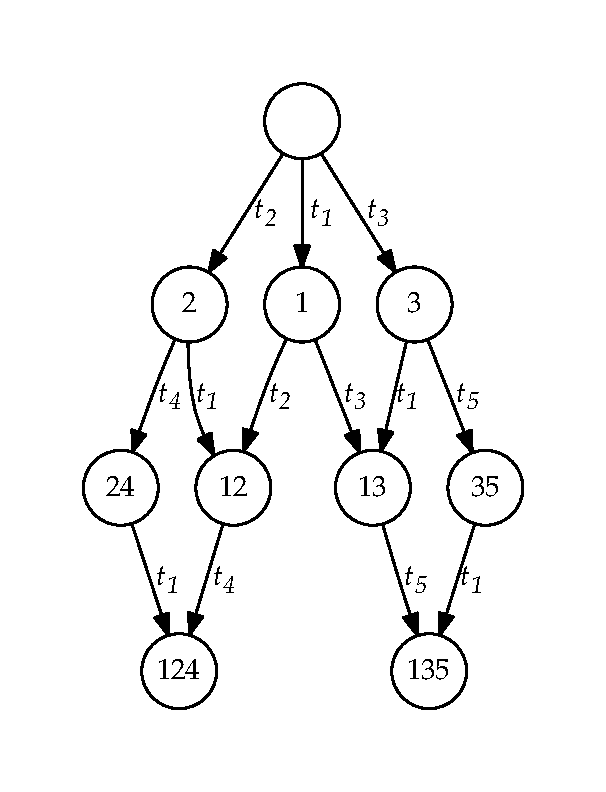
\includegraphics[height=9cm]{persistent1}
		\caption[Diagram of an example state space, for
		the illustration of persistent sets.]
		{Diagram of an example state space, for
			the illustration of persistent sets. Transition
			$t_1$ is independent with the others, which are
			all dependent with one another.}
		\label{fig:persistent}
	\end{minipage}%
	\qquad
	\begin{minipage}{.45\textwidth}
		\centering
		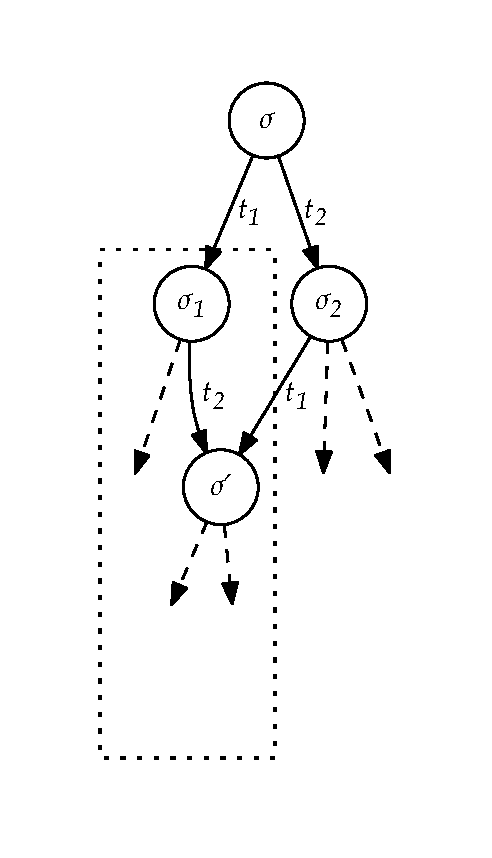
\includegraphics[height=9cm]{sleep}
		\caption{Diagram illustrating the
			idea behind sleep sets.}
		\label{fig:sleep}
	\end{minipage}
	
\end{figure}

\subsection{Sleep Sets}
\label{sec:sleep-prep}

Another technique that addresses
the state explosion problem is
that of \emph{sleep sets}, again by Godefroid \cite{god91}.
Suppose that
we are at state $\sigma$ when performing a search
of the state space (see Figure~\ref{fig:sleep}).
Suppose we first explore $t_1$, reaching $\sigma_1$,
and then $t_2$, reaching $\sigma_2$.
If $t_1$ and $t_2$ are independent, then there
is a state $\sigma'$ reachable by both
$\sigma \xrightarrow{t_1} \sigma_1
\xrightarrow{t_2} \sigma'$ and
$\sigma \xrightarrow{t_2} \sigma_2
\xrightarrow{t_1} \sigma'$.
Clearly, any stopped state reachable from $\sigma'$
is reachable from $\sigma_1$. By assumption,
when the search is at $\sigma_2$, we have already
explored all the stopped states reachable from
$\sigma_1$ (the dotted area in Figure~\ref{fig:sleep}),
in particular those reachable from
$\sigma'$. Therefore, there is no need to
explore $t_1$ from $\sigma_2$.

In fact, there is no need to consider executing
$t_1$ in our recursive exploration from $\sigma_2$
until we execute some transition $t'$ which is
\emph{not} independent with $t_1$, since only after
the execution of such a $t'$ may exploring $t_1$
then lead to an unexplored area of the state space.

A sleep-set algorithm is one that maintains a
set of transitions which, by the above argument,
need not be explored from the current state.

\section{Dynamic Partial-Order Reduction}
\label{sec:dpor-prep}
After reading this section, you should
understand roughly how the dynamic
partial-order reduction algorithm works.
The information in this section is
adapted from the POPL paper \cite{flan05}.

\subsection{Background Definitions}

\subsubsection{Transition Sequences}
Instead of keeping track of just the current state,
the DPOR algorithm
keeps track of a \emph{transition
sequence} $\pi \in \mathcal{T}^*$. This transition
sequence is implicitly executed from the initial state of
the transition system, $\sigma_0$, so that in practice,
$\pi = t_0, t_1, \ldots, t_{n-1}$ determines a sequence of states
$\sigma_0, \sigma_1, \ldots, \sigma_n$ such that
\[
	\sigma_0 \xrightarrow{\ t_0\ } \sigma_1 \xrightarrow{\ t_1\ }
	\ldots \xrightarrow{t_{n-1}} \sigma_n.
\]

Given a transition sequence $\pi = t_0, t_1, \ldots, t_{n-1}$,
we use the following notation:
\begin{itemize}[label={}]
	\newcommand{\defsindent}{3.5em}
	\item{\makebox[\defsindent]{\hfill$\pi_i$}
		--- the transition $t_i$;}
	\item{\makebox[\defsindent]{\hfill$\pi.t$}
		--- the transition sequence $\pi$ extended with
		transition $t$;}
	\item{\makebox[\defsindent]{\hfill$\textit{dom}(\pi)$}
		--- the set $\{i \in \mathbb{N} \mid 0 \leq i < n \}$;}
	\item{\makebox[\defsindent]{\hfill$|\pi|$}
		--- the length of the transition sequence, $n$;}
	\item{\makebox[\defsindent]{\hfill$\textit{pre}(\pi, i)$}
		--- the state $\sigma_i$ immediately preceding $\pi_i$; and}
	\item{\makebox[\defsindent]{\hfill$\textit{last}(\pi)$}
		--- the final state, $\sigma_n$.}
\end{itemize}

\subsubsection{The Happens-Before Relations}\label{sec:happens-before}

Suppose that two adjacent transitions, $\pi_i$ and $\pi_{i+1}$,
are swapped in a
transition sequence $\pi$ to give a new
transition sequence, and that
$\pi_i$ and $\pi_{i+1}$ are independent.
Because the order of execution of a
pair of independent transitions is
irrelevant in the sense that it
results in the same state, the result
of executing the two transition
sequences must be the same
(see Figure~\ref{fig:sequence-equivalence}).
It follows that any transition sequence obtained
by making a finite number of swaps of adjacent
independent transitions is equivalent in the same
sense. Such equivalence classes are known as
Mazurkiewicz traces \cite{maz87}, and are
the basis of DPOR, since it is
sufficient to explore only one member of
each equivalence class.

\begin{figure}[b]
	\centering
	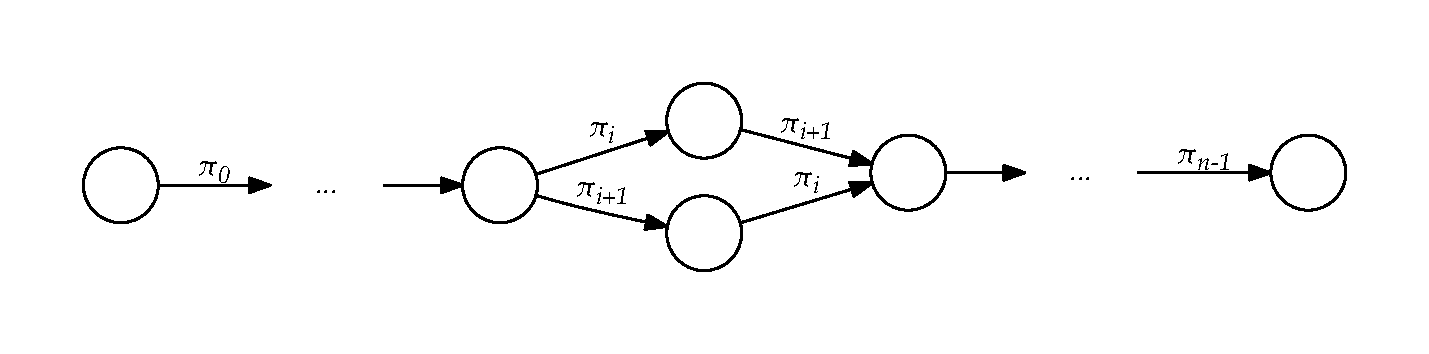
\includegraphics[width=\textwidth]{seqequiv}
	\caption{Illustration of equivalent transition sequences.}
	\label{fig:sequence-equivalence}
\end{figure}

It is useful to consider a
``happens-before'' relation that identifies
pairs of transitions which
cannot be swapped with one another
to form an equivalent sequence.
In particular, the \emph{happens-before}
relation $\longrightarrow_\pi$ for a transition
sequence $\pi$ is the smallest relation on
$\textit{dom}(\pi)$ such that
\begin{enumerate}
	\item if $i \leq j$ and $\pi_i$ is dependent with
		$\pi_j$ then $i \longrightarrow_\pi j$, and
	\item $\longrightarrow_\pi$ is transitively closed.
\end{enumerate}
By construction, the happens-before relation is a
partial-order relation on the transitions in $\pi$,
and the linearisations of $\longrightarrow_\pi$
are precisely the transition sequences equivalent
to $\pi$.

The DPOR algorithm makes use of a variant of the
happens-before relation, which guarantees that a
process must execute its next transition by the
end of the current transition sequence.
Informally, if $i \hookrightarrow_\pi p$ then
for some $j \geq i$,
the process of $\pi_j$ 
is $p$, both in $\pi$ and any
equivalent transition sequence.
Formally, 
if $i \in \textit{dom}(\pi)$ and $p \in
\mathcal{P}$ then $i \hookrightarrow_\pi p$ if
either
\begin{enumerate}
	\item $\textit{proc}(\pi_i) = p$, or
	\item $\exists j \in \textit{dom}(\pi).\;
	i < j \,\wedge\, \textit{proc}(\pi_j) = p
	\,\wedge\, i \longrightarrow_\pi j $.
\end{enumerate}


\subsection{The Dynamic Partial-Order Reduction Algorithm}

The DPOR algorithm
uses information gathered dynamically during its
exploration of a state space to explore only
transitions in a persistent set from each state
encountered on the search. The idea is that the
extra information allows smaller
persistent sets to be computed than would
otherwise be possible, thereby making the
search more efficient.

In particular, at each state $\sigma$, the
next transition
to execute, $t$, is chosen arbitrarily, and it is
initially assumed that $t$ will
be the only transition to be explored from
that state. However, $\{t\}$ is a persistent
set only if $t$ is
independent of every transition reachable
by exploring any transitions
from $\sigma$ other than $t$. Clearly,
this is not true in general, so at each
state $\sigma'$ encountered beyond
$\sigma$, if there is a transition
$t' \in \textit{enabled}(\sigma')$
such that $t'$ is dependent with
$t$, and $t'$ may appear before $t$
in an exploration from $\sigma$, then
a backtracking point is added at
$\sigma$ to ensure that such an
exploration is made.
The addition of such backtracking points
ensures that the set of transitions
explored from each state is a
persistent set.

The pseudocode for and a more
detailed explanation of the DPOR
algorithm are provided in
Appendix~\ref{app:dpor-walkthrough}.

\newcommand{\dporpseudocode}{
	\begin{algorithmic}[1]
		\Procedure{Explore}{$\pi$}
		\Let{$\sigma$}{$\textit{last}(\pi)$}
		\ForAll{$p \in \mathcal{P}$}
		\State \Call{UpdateBacktrackSets}
		{$\pi,\, \textit{next}(\sigma, p)$}
		\EndFor
		\If{$\textit{enabled}(\sigma) \neq \emptyset$}
		\Let{$t$}{any $t \in \textit{enabled}(\sigma)$}
		\Let{$\textit{backtrack}(\sigma)$}{$\{t\}$}
		\Let{$\textit{done}(\sigma)$}{$\emptyset$}
		\While{$\textit{done}(\sigma)
			 \neq \textit{backtrack}(\sigma)$}
		\Let{$t$}{any $t \in (\textit{backtrack}(\sigma)
			\setminus \textit{done}(\sigma))$}
		\State add $t$ to $\textit{done}(\sigma);$
		\State \Call{Explore}{$\pi.t$}

		\EndWhile
		\EndIf
		\EndProcedure
		\State
		\Procedure{UpdateBacktrackSets}{$\pi,\, t_{p,s}$}
		\Let{$D$}{$\{i \in \textit{dom}(\pi) \mid
			\pi_i \text{ is dependent with } t_{p,s}
			\text{ and } i \not \hookrightarrow_\pi p\}$}
		\If{$D \neq \emptyset$}
		\Let{$\sigma_d$}
		{$\textit{pre}(\pi,\text{max}(D))$}
		\If{$\textit{next}(\sigma_d, p)
			\in \textit{enabled}(\sigma_d)$}
		add $\textit{next}(\sigma_d, p)$
		to $\textit{backtrack}(\sigma_d)$
		\Else {
			add all of $\textit{enabled}(\sigma_d)$
			to $\textit{backtrack}(\sigma_d)$
		} \EndIf
		\EndIf
		\EndProcedure
		\State
		\State Initially: \Call{Explore}{$\emptyset$}
	\end{algorithmic}
}

\chapter{Implementation}
\label{cha:imp}
After reading this chapter,
you should understand:
\begin{understandinglist}
	\item the software development approach
	I used;
	\item the high-level structure and
	organisation of my project;
	\item the design and implementation of
	the programming language used
	as the object language for the
	project;
	\item the details of my
	implementation of the DPOR algorithm; and
	\item how I implemented some other
	model-checking algorithms.
\end{understandinglist}


\section{Software Engineering}
After reading this section, you should
understand how I approached the
development of my project, and what its high-level
structure is.

\subsection{Development Strategy}
I used an
incremental approach to the
development of my project.
This involved breaking down 
the project into several
subgoals, each of which I implemented
and tested in turn, before moving on to the next.
The subgoals were
to:
\begin{itemize}
	\item design a concurrent programming
	language and create an interpreter for it;
	\item create a parser for that language;
	\item implement a simple model-checking
	algorithm;
	\item implement DPOR, assuming
	a language without locks for simplicity; and
	\item add locks to the DPOR implementation.
\end{itemize}
Each of the several extensions I completed
was also developed as a new incremental subgoal.

The benefits of this approach include the frequent
testing of each new component, the manageable
size of each subgoal, and the creation of
working software from the beginning.

\subsection{Structure of the Project}
The project was implemented in OCaml, which
offers a few key advantages:
\begin{itemize}
	\item a clean, functional
	style;
	\item a strong, safe type system, which prevents
	a large class of runtime errors;
	\item parametric polymorphism, a module system,
	and other higher-order programming features,
	facilitating abstraction and generalisation; and
	\item established libraries, providing efficient
	implementations of basic data structures and algorithms.
\end{itemize}

OCaml modules
provide abstraction by encapsulating
related definitions and hiding implementation details.
\emph{Signatures} are software interfaces
providing declarations,
and \emph{structures} are implementations which 
provide definitions. A structure \emph{matches} a
signature if it has a definition for each declaration
in the signature. \emph{Functors} act as
functions between modules.

\begin{figure}
	\centering
	\begin{minipage}{.47\textwidth}
		\centering
		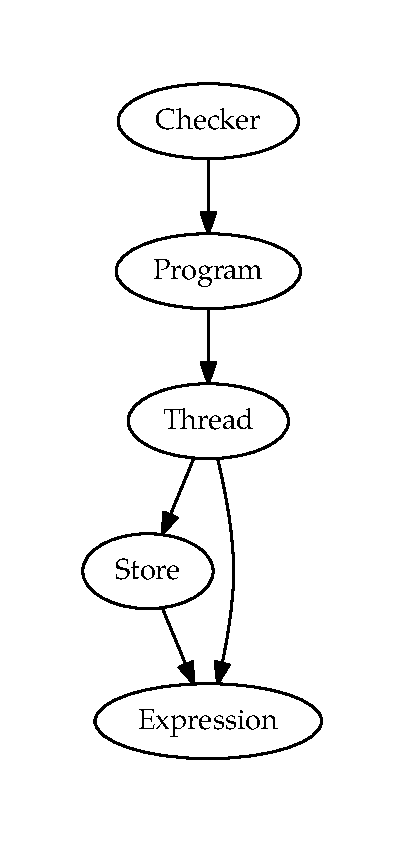
\includegraphics[height=11cm]{interfaces}
		\caption{Diagram showing which signatures declare
			which other signatures as nested sub-structures.}
		\label{fig:interfaces}
	\end{minipage}%
	\qquad
	\begin{minipage}{.47\textwidth}
		\centering
		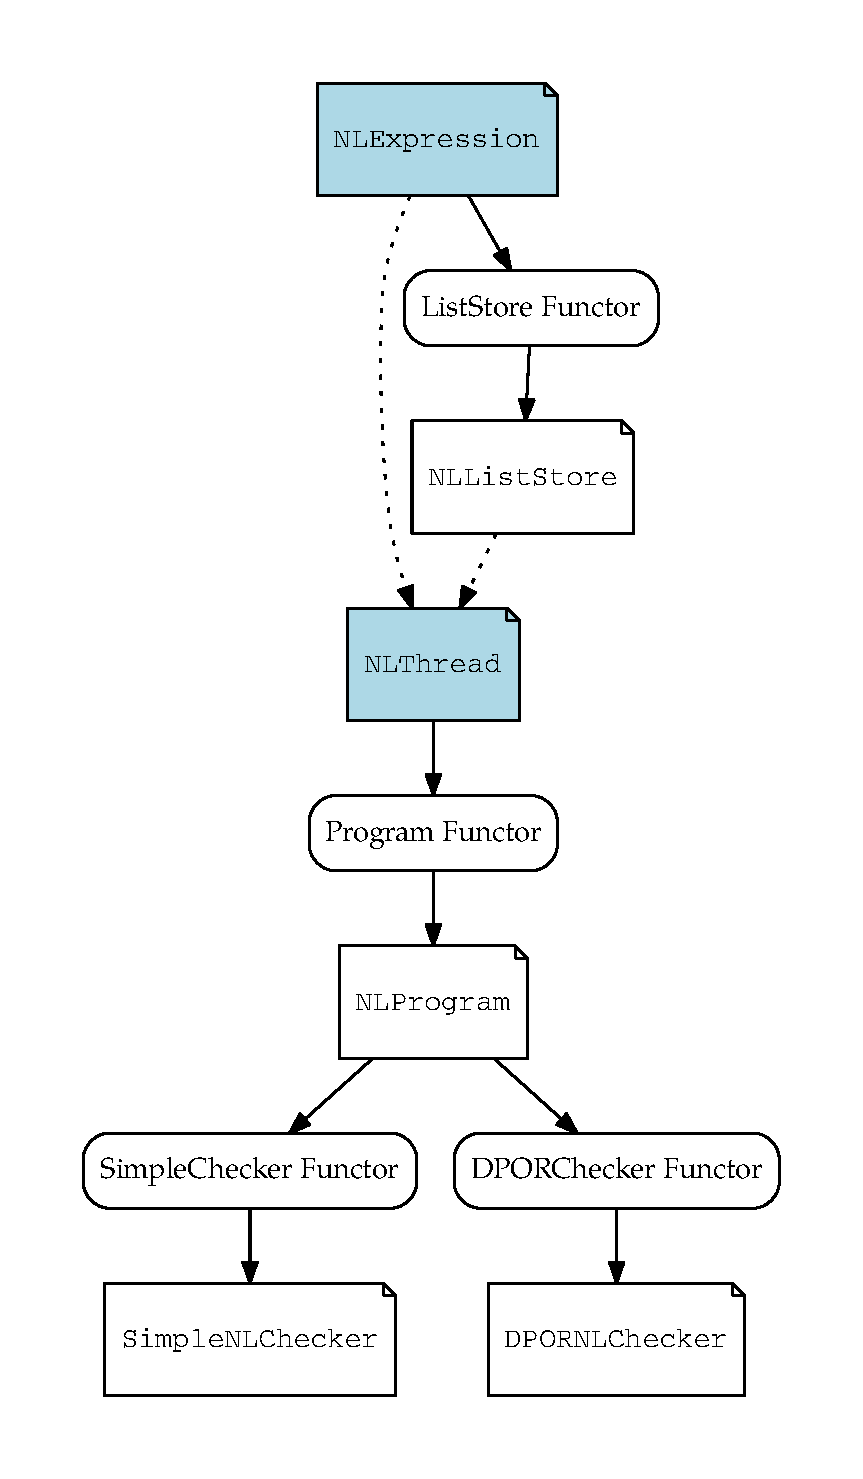
\includegraphics[height=15cm]{functors}
		\caption{Diagram showing generation of
			structures using functors.
			The shaded files must be provided,
			the functors are part of my project,
			and the remaining files
			are generated using the functors.}
		\label{fig:functors}
	\end{minipage}
\end{figure}

In my project, there are five main signatures:
\begin{enumerate}
	\item \emph{Expression}	contains information
	about the structure of expressions
	in the programming language of interest;
	\item \emph{Store} implements
	a mapping from locations
	to expressions for some
	implementation of \emph{Expression};
	\item \emph{Thread} contains the
	information about the reduction of
	expressions for one thread;
	\item \emph{Program} contains declarations
	combining threads to express a full concurrent
	program; and
	\item \emph{Checker} declares a function
	which performs model checking on a given
	concurrent program.
\end{enumerate}

Since model checking is independent of any
particular programming language, I used functors
to minimise the work needed to use my project
for a new language.
From two structures matching \emph{Expression} and \emph{Thread},
functors automatically generate implementations of
\emph{Store}, \emph{Program} and \emph{Checker},
because I wrote
each model-checking algorithm as a functor.
A working implementation of each model-checking
algorithm in my project can therefore be
obtained for a new language just by
specifying its syntax and semantics.
This process is shown explicitly in
Figure~\ref{fig:functors} for
a hypothetical new language, NL.


\section{Development of the Project Language}
\label{sec:language}
After reading this section, you should
understand how I designed
and implemented a programming
language for the expression
of programs to model check.

\subsection{Language Design}
Although any concurrent
thread-based programming language
could be used to express transition systems for model
checking, I chose to design and implement a simple
ML-like language, PL (Project Language), to avoid
dealing with the full complexity of an
industrial language. When designing PL, my aim
was to create a high-level language that had enough features
to easily write practical concurrent programs,
but was not unnecessarily complex.

PL is a Turing-complete functional
language which operates on integers,
Booleans and first-class functions.
Thread-local reference cells provide some
procedural functionality, and the usual
structures manage flow control. There is
an error construct, which allows easy syntactic
checking of whether a thread has encountered
an error. The shared
state is a collection of variables that are
shared between all threads, some of which
can be locks, used to enforce mutual exclusion.
There are four atomic operations
that interact with shared variables:
\begin{enumerate}
	\item a read operation returns the current value
	of a shared variable;
	\item a compare-and-swap operation
	compares the value of a shared variable to a
	given value, and if they are the same, updates
	the shared variable to another given value and returns
	``true'', else it returns ``false'';
	\item a lock operation takes the given lock if
	available, else blocks until it becomes available; and
	\item an unlock operation makes the given lock
	available.
\end{enumerate}
Since the locking operation is the only
one that can block, it is a trivial syntactic
check to decide whether a given thread is
blocked or not.

I did not write a type system for PL because
I thought that the time to implement one would
be greater than the time saved as a result. In hindsight,
I think this was correct.

\subsection{Parser}
I decided that investing time in creating a
parser for PL would pay itself off over the course of the project.
A parser allowed me to write, for example,
\begin{align*}
	\texttt{let y = ref 1 in cas(Gx, 7 * !y - 3, 0)},
\end{align*}
instead of having to type the OCaml meta-language abstract
syntax tree representing the structure of the PL expression,
\begin{align*}
	\texttt{Let (Ref (Integer}& \texttt{ 1), Cas (Global "x",
		Op (Op (Integer 7,} \\ \texttt{Mult,}& \texttt{ Deref (Var 0)), Minus, Integer 3),
		Integer 0))}.
\end{align*}
Writing such expressions is not only extremely time-consuming but
also error-prone. For the language to be of any practical use,
a parser was a necessity.

To create a parser for PL, two program generators were used:
OCamllex and Menhir. When given a
file detailing a mapping from strings of characters to tokens,
OCamllex produces a lexical analyser, which converts a sequence
of characters into a sequence of tokens. When given a
grammar and a set of precedence rules, Menhir produces a parser,
which converts a sequence of tokens into an abstract syntax tree
of the grammar. These were used in conjunction, as shown in
Figure~\ref{fig:parsing}, to produce a full parser for PL.

\begin{figure}
	\centering
	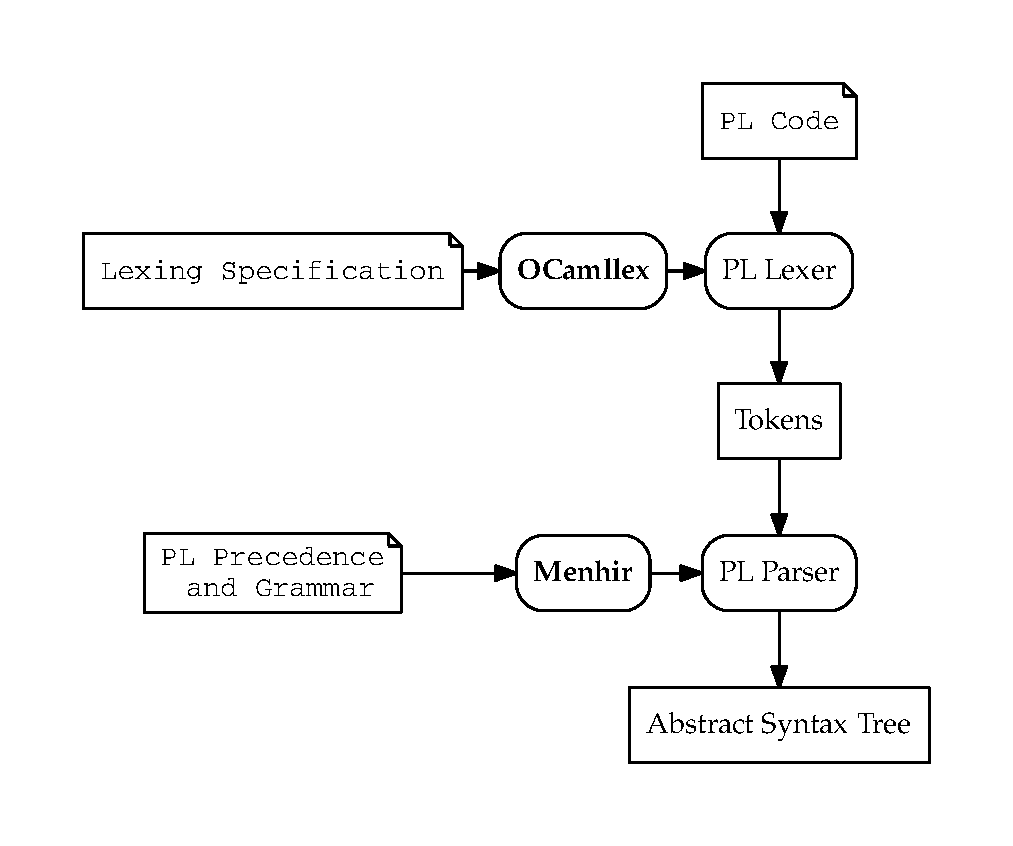
\includegraphics[height=10cm]{parsing}
	\caption{Diagram showing the parsing of
		a PL program.}
	\label{fig:parsing}
\end{figure}

\subsection{Implementation}

\subsubsection{The Expression Module}
Two datatypes are used to
represent PL expressions: a ``raw'' expression, which
uses strings to represent variables (this is the
datatype that the parser produces), and a datatype
which uses De Bruijn indices \cite{debr72} to
represent variables, allowing
easier manipulation of expressions.

The remainder of the \emph{Expression} module
consists mainly of auxiliary functions which are
necessary for the implementation of later
modules, and either return a simple piece
of information or perform a simple manipulation.

\subsubsection{The Store Module}
A functor, ListStore, is used. Given an
\emph{Expression} implementation, it
returns a \emph{Store} implementation, which
represents stores using lists of
(location,~expression) pairs. Mappings
are adding by appending a new pair to
the front of the list, causing any old
mapping for that location to become stale.
A function is provided that walks through
the list removing stale pairs, used to
prevent the list from growing too long,
or in situations when there must be
no stale values in the list.

More efficient store implementations are
possible---for example, one based on
a hash table rather than a list---but
I valued simplicity over efficiency
in this case,
to increase my confidence in its correctness.

\subsubsection{The Thread Module}
The \emph{Thread} module consists primarily of
the \texttt{next\_step} and \texttt{next\_transition}
functions, which define the semantics of PL.
Given an expression, \texttt{next\_step} uses pattern
matching to determine what the next atomic
operation (if any) is for the reduction
of that expression.
Care must be taken to
ensure that each step given here really is
atomic, else race conditions could exist
in real executions of programs that would
not be found by model checking. This
is not a concern for PL, since its only
implementation is the one used for the
model checker, but would be if
an industrial language was used.

Given the definition
of a transition (cf.\@ Section~\ref{sec:trans-prep}),
the \texttt{next\_transition}
function repeatedly calls the \texttt{next\_step}
function until some step accesses the shared
store, at which point the resulting expression
and updates to the stores are returned.

\subsubsection{The Program Module}
The \emph{Program} module is a small functor which,
when given a \emph{Thread} implementation, provides 
the few additional definitions and auxiliary
functions necessary to fully represent the state of
transition systems (cf.\@ Section~\ref{sec:background-defs}).
In particular, a state $\sigma \in \textit{State}$ is
represented by an instance of the \texttt{state} type:
\lstinputlisting[frame=none, firstline=121, lastline=121]
	{../src/interfaces.ml}

\subsubsection{Testing}
To ensure that the implementation of the PL
language was correct, I wrote around
twenty unit tests for
the \texttt{next\_transition} and
\texttt{next\_step} functions. These had good
code coverage, and caught most of the bugs I
found in the implementation of PL.


\section{Dynamic Partial-Order Reduction}
An overview of the DPOR
algorithm was given in Section~\ref{sec:dpor-prep},
with a more detailed explanation
given in Appendix~\ref{app:dpor-walkthrough}.
Several aspects of the implementation of DPOR
are not obvious; after reading this section
you should understand how I implemented
all aspects of DPOR.

\begin{figure}[h]
	\dporpseudocode
	\caption{The DPOR algorithm.}
	\label{fig:dpor-imp-pscode}
\end{figure}

\subsection{Implementation}
This section explains how I translated
the pseudocode in Figure~\ref{fig:dpor-imp-pscode}
into an executable OCaml function, \texttt{check},
which is given in Appendix~\ref{sapp:dpor-imp}
for reference.

\begin{description}
	\item[Line 2] When implementing the simple
	model checker (cf.\@ Section~\ref{sec:simple-imp}),
	I used the \texttt{fold\_left}
	function from the library List module to
	repeatedly use the \texttt{apply\_transition}
	from the \textit{Program} module to apply
	the transitions in the transition sequence
	to the initial state. However, in this case
	I wrote a more general function, \texttt{pre},
	which applies only the first
	$n$ transitions in the sequence,
	thereby returning the state
	$\textit{pre}(\pi, n)$ if $n < |\pi|$
	or the state $\textit{last}(\pi)$ if
	$n = |\pi|$, which is what we want in
	this case.

	\item[Lines 3--4] The \texttt{next\_transition}
	function, provided in the \textit{Thread} module,
	may return no transition at all (for instance
	in the case that a thread has terminated its
	computation), so the call to 
	\textsc{UpdateBacktrackSets} is only made if
	\texttt{next\_transition} does return a
	transition.

	\item[Lines 15--17] In my project,
	each transition $t$ accesses only one shared
	object, denoted $\alpha(t)$,
	and it is assumed that two transitions are
	dependent if and only if they access
	the same shared object (or belong to the
	same process). It follows that the most
	recent transition $\pi_i$ such that
	$\pi_i$ is dependent with $t_{p,s}$
	and $i \not\hookrightarrow_\pi p$,
	if any,
	is precisely the last transition
	to access $\alpha(t_{p,s})$.

	Therefore, as well as the transition
	sequence, $\pi$, \texttt{check} takes
	as an argument 
	a function $L$, such that $L(o)$ is the
	index of the last transition that accessed
	shared object $o$, so that the index of the
	necessary backtracking point, if any, is
	$L(\alpha(t_{p,s}))$. However, if
	this transition happens-before
	$t$ then no backtracking point at all
	is necessary, since there cannot be another
	transition that is dependent with $t$
	but does not happen-before $t$. To
	decide the happens-before relation,
	clock vectors are used, as described 
	in Section~\ref{sec:clock-vectors}.

	Because	$\sigma_d = pre(\pi, L(\alpha(t_{p,s})))$,
	the \texttt{pre} function mentioned above can be
	used to obtain $\sigma_d$.

	\item[Lines 18--19]	The \texttt{next\_transition} function
	returns a Boolean with each transition, indicating whether
	it is enabled in the given state, so that deciding whether
	$\textit{next}(\sigma_d,p)$ is enabled is trivial.
	This also
	means it is easy to compute the enabled
	set of a state, by iterating through the processes
	and looking at whether the next transition of each
	is enabled.
	
	\item[Lines 5--6] If, while iterating through the
	processes in lines 3 and 4, any transition is found to be
	enabled, then a reference is set to it. If at line 5,
	that reference has been set at all, then it is chosen
	as the $t \in \textit{enabled}(\sigma)$ in line 6,
	otherwise lines 6 to 12 are not executed.

	\item[Line 7] The \textit{backtrack} sets for each state
	in the sequence of states implied by the transition
	sequence $\pi$ must be stored in a data structure that
	allows them to be accessed and updated from all later
	recursive calls, so that they can add backtracking
	points. I decided to use a variable-length array
	for this, as arrays are mutable and have efficient
	access, but the maximum recursion depth (and so the
	longest fixed-length array necessary) cannot be predicted.
	
	I therefore implemented a module which uses a fixed-length
	array to implement a variable-length array by
	copying the elements to a fresh array of double the
	previous size if the underlying array proves too short.
	Although this operation is expensive, the amortised
	cost of adding a new element to the array is constant.
	In this case, each element of the array is a \textit{backtrack}
	set of a state, implemented as a list of processes
	whose next transitions are to be explored.
	
	\item[Lines 8--11] Instead of using a
	procedural while-loop,
	I implemented the iteration through
	the backtracking points
	using a tail-recursive
	function, taking a list of processes
	representing the \textit{done} set as
	its argument. An auxiliary
	function returned a member $p$ of the
	\textit{backtrack} set not present in the
	\textit{done} set, from which the
	transition $t$ to explore is simply
	$\textit{next}(\sigma, p)$. The
	recursive call to the tail-recursive function
	then has the old \textit{done} set
	extended with $p$ as its argument. If
	the auxiliary function can
	find no such $p$, then the
	tail-recursive function (and therefore the
	call to \texttt{check}) returns.

	\item[Line 12] Once the new arguments have
	been computed, a recursive call to
	\texttt{check} is made. Other than
	the clock vectors (see Section~\ref{sec:clock-vectors}),
	the arguments that
	have to be computed are the new transition
	sequence, $\pi' = \pi.t$,
	and the new function, $L'$,
	tracking which transitions have accessed each 
	object:
	\[ L'(o) =
	\begin{cases}
		\hfill |\pi| \hfill & \text{ if } o = \alpha(t); \\
		\hfill L(o) \hfill & \text{ otherwise}.
	\end{cases}\]

	\item[Line 13] Once all backtracking points have been
	explored, the result is returned.
	Appendix~\ref{sapp:simple-code} explains
	how errors and deadlocks are
	detected in the simple model checker,
	and the computation is very similar
	for the DPOR algorithm. The iteration
	through all threads on line 3 is used
	to also check whether any thread has
	encountered an error, is enabled,
	or is blocked.
	This information is combined with the
	results from the recursive calls to
	compute whether the state space from
	the current state onwards is error-free
	and deadlock-free.

\end{description}

\subsection{Deciding The Happens-Before Relation}
\label{sec:clock-vectors}

To decide the happens-before relation,
$\hookrightarrow_\pi$, I used clock vectors.
Although Flanagan
and Godefroid outline how clock vectors
can be used \cite{flan05},
they do not give the
following detail in the
reasoning.

\subsubsection{Using Clock Vectors}

As explained above, although
the function $L$ gives the index
of the last transition that accessed a given shared
object, which is the index of the potential backtracking
point, we only need to add it if it
did not happen-before the current transition.
That is, if
$L(\alpha(t_{p,s})) \not\hookrightarrow_\pi p$.

If, for each process
$q$, we know the index $k$ of the last transition of that
process such that $k \hookrightarrow_\pi p$,
then given any other transition $\pi_i$ of
process $q$, we know that
$i \hookrightarrow_\pi p$ if and only if
$i \leq k$. A clock vector $c$ is
a function from processes $q$ to such
indices $k$ in the transition sequence,
and we maintain one clock vector, $c_p$, per
process $p$. To decide whether
$i \hookrightarrow_\pi p$ for
any $i$ and $p$ is simply to decide
whether $i \leq c_p(q)$, where $q$ is
the process of transition $\pi_i$.
This takes constant time.

\subsubsection{Updating Process Clock Vectors}
By passing correct clock vectors as arguments to
\texttt{check}, then, it is straightforward
to decide whether we need to add each potential
backtracking point.
Assuming that the correct value is passed for
the initial call,
(namely each $c_p(q) < 0$)
we need to ensure that the
clock vectors are correctly updated when
a recursive call exploring a new transition,
$t_{p,s}$, is made.

The only clock vector that needs to be updated
is $c_p$, since $i \hookrightarrow_\pi p'$ if
and only if $i \hookrightarrow_{\pi'} p'$,
where $\pi' = \pi.t_{p,s}$ and $p' \neq p$.
Let us denote the updated clock vector
by $c_p'$, and consider $c_p'(q)$, which
must be at least $c_p(q)$, because if process
$p$ must happen-before the end of $\pi$
then it must happen-before the end of $\pi'$.
However, if there is a more recent transition
of process $q$, say $\pi_i$
that accesses the same shared
object as the new transition $t_{p,s}$, then
$c_p'(q)$ must be updated to the index of
that transition, because $\pi_i$ must
happen-before $t_{p,s}$.

To perform this update, we need to keep
track of the index $k$ of the most recent
transition of each process $p$ that
accesses each shared object $o$. We therefore
also maintain a clock vector $c_o$ for each
shared object $o$, and set
\[ c_p'(q) =\textit{max}(c_p(q),
		c_{\alpha(t_{p,s})}(q)).\]
The only special case is when $q = p$,
in which case $c_p'(p) = |\pi|$, since
the last transition is now a transition of
process $p$, and $|\pi|$ is the index
of the last transition in $\pi'$. The
full update for the clock vector is therefore
\[ c_p'(q) =
\begin{cases}
	\hfill |\pi| \hfill & \text{ if } q = p; \\
	\hfill \textit{max}(c_p(q),
		c_{\alpha(t_{p,s})}(q))
		\hfill & \text{ if } q \neq p.
\end{cases}\]


\subsubsection{Updating Object Clock Vectors}

We have seen how to use object clock vectors to
update the process clock vectors, but
the object clock vectors themselves must also be
updated whenever a new transition is explored.
In particular, if the clock vector for the
object accessed by the transition must be
updated so that the thread of the transition
maps to that transition:
\[c_{\alpha(t_{p,s})}'(p) = |\pi|.\]

However, we can do better, by letting
$c_o(q)$ be the index of the
last transition of process
$q$ such that object $o$ is guaranteed to be
accessed between $c_o(q)$ and the last
transition of the sequence (inclusive),
whether or not $\pi_{c_o(q)}$ itself
accesses $o$.
This is sufficient for updating the
process clock vectors as above, and
also allows for higher indices to
be stored than just the last
transition of a process that
accesses the object.

For example, suppose that,
for some process $q \neq p$,
$c_{\alpha(t_{p,s})}(q) < c_p(q)$. That is,
more recently than the last transition of
$q$ that accessed the object $\alpha(t_{p,s})$,
there was a transition of $q$ that happens-before
some transition of process $p$ prior to the new
transition $t_{p,s}$. Since any previous
transition of process $p$ must happen-before
$t_{p,s}$, we know that the transition
of index $c_p(q)$ must also happen-before
$t_{p,s}$. Therefore, there is a transition
(namely $t_{p,s}$) which
accesses $\alpha(t_{p,s})$ and is guaranteed
to happen after $\pi_{c_p(q)}$. So we can
safely perform the following update:
\[ c_{\alpha(t_{p,s})}'(q) =\textit{max}(c_p(q),
c_{\alpha(t_{p,s})}(q)),
\]
meaning that the full update for the object
clock vector is

\[ c_{\alpha(t_{p,s})}'(q) =
\begin{cases}
\hfill |\pi| \hfill & \text{ if } q = p; \\
\hfill \textit{max}(c_p(q),
c_{\alpha(t_{p,s})}(q))
\hfill & \text{ if } q \neq p.
\end{cases}\]

Noting that this is precisely the same
clock vector as $c_p'$ allows for a
more efficient implementation of
the updates.

\section{Counter-Example Traces} \label{sec:traces}
One of the advantages of model checking
is that, if
an error is found, it is easy to
give an example execution leading
to that error---in
our case, this is just the sequence of
transitions leading to the error state.
To give more insight into the reason for the
error state being entered, the user could
instead be given a
\emph{partial order} of the transitions which,
whenever linearised into an execution,
results in the error (or deadlock) state.

This partial order is simply the happens-before
relation, as described in
Section~\ref{sec:happens-before}. As
two transitions are dependent if and only
if they belong to the same thread or if
they access the same shared object, my
algorithm executes the given transition
sequence, using functions from processes
and shared objects to positions in
the sequence to track the last
transition to each process and
to access each shared object respectively.
For each
transition executed, two ``happens-before''
edges are added
to a graph representing the partial
order: one from the last transition
belonging to the same process, and one
from the last transition accessing the
same shared object.

To show the partial order graph in an
easily-interpretable way, I
output a GraphViz file displaying the
graph, with each node
labelled with its process and the
shared object it accesses.
GraphViz is an open-source program which
draws graphs.
Figure~\ref{fig:trace-example}
shows an example of such an
automatically-generated graph.

\begin{figure}
	\centering
	\begin{subfigure}{0.5\textwidth}
		\centering
		\begin{tabular}{l}
			Shared variables: \\
			\qquad \texttt{n}, \texttt{w},
			\texttt{x} and \texttt{y},
			initially \texttt{0} \\
			\qquad \texttt{t} and \texttt{z},
			initially \texttt{false} \\
			\\
			Thread 0: \\
			\qquad \texttt{t := z;} \\
			\qquad \texttt{if t then x := y} \\
			\\
			Thread 1: \\
			\qquad \texttt{n := 1;} \\
			\qquad \texttt{z := true} \\
			\\
			Thread 2: \\
			\qquad \texttt{y := 2;} \\
			\qquad \texttt{if w = 1 \& x = 2 then \textbf{error}} \\
			\\
			Thread 3: \\
			\qquad \texttt{w := n} \\
			\\
			Thread 4: \\
			\qquad \texttt{t := false} \\
		\end{tabular}
	\end{subfigure}%
	\begin{subfigure}{0.5\textwidth}
		\centering
		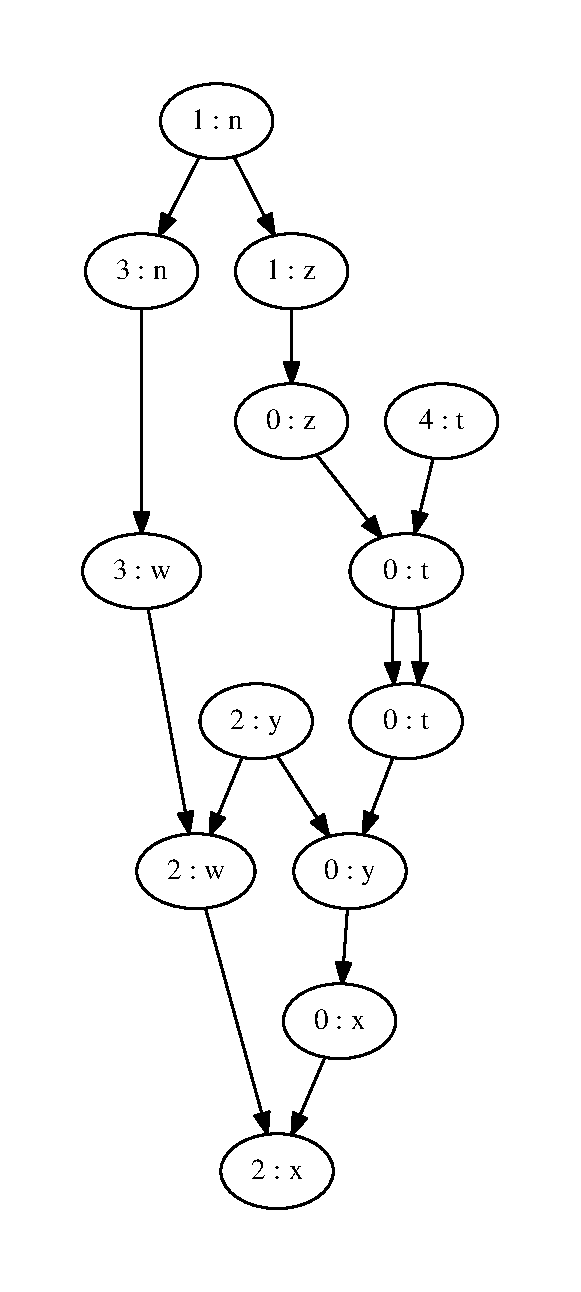
\includegraphics[height=15cm]{error_trace}
	\end{subfigure}
	\caption[An example partial-order
	error trace.]{An example partial-order
		error trace. The assignments in
		the program are implemented in PL
		using compare-and-swap operations.}
	\label{fig:trace-example}
\end{figure}

\section{Extensions For Evaluation}
Having reached my goal of implementing
the DPOR algorithm, I decided to
implement some additional model-checking
algorithms as extensions, to allow a
comparative evaluation of their
performances. After reading this
section, you should understand how
I implemented these other model-checking
algorithms.

\subsection{Simple Model Checker}
\label{sec:simple-imp}
Implementing and testing
the simple model checker
before DPOR
(although not an extension)
allowed me to
sanity-check my PL implementation,
practise with an easy
model-checking algorithm first,
and later verify the results of
my DPOR implementation.
It also provides a performance
baseline for the evaluation of
the other algorithms.
As outlined in
Section~\ref{sec:simple-prep}, it
performs an exhaustive depth-first
search of the state space,
recursively deciding whether each
state is error-free
and deadlock-free.
Appendix~\ref{sapp:simple-code} gives
the pseudocode for this algorithm,
and explains how it is decided whether
an error or deadlock state has been reached.

\subsection{Stateful Model Checking}
If we keep track of which states we have
already explored on a search, then when
we re-encounter a state, we can cut short
the search in the knowledge that we have
already explored from that state, improving
time efficiency at the cost of extra space.

\subsubsection{Simple Model Checker}

Applying this technique to the simple model
checking algorithm is straightforward: whenever
a state is visited, add it to some data structure,
then explore only those states which are not
present in that data structure. As querying
this structure and inserting a state to it
happens at every state, we would like these
operations to be efficient. The typical amortised costs
of both these operations for a hash table are
constant, so I used the OCaml library implementation
of hash tables for this purpose.

\subsubsection{Dynamic Partial-Order Reduction}
Suppose that we applied this approach
to the DPOR algorithm,
and executed the resulting algorithm
on the example shown in
Figure~\ref{fig:sdpor-motivation}.
Consider the stage at which
all the states in grey have been
explored and so are present in the hash table,
and the current transition sequence is the first
transition of thread 1 followed by the first
transition of thread 0. As this stage, the state
labelled 2200 is encountered, which is already
present in the hash table, so no exploration is
made, and as no backtracking points have been added
at either of the previous stages, the algorithm
terminates.

However, this leaves part of the state
space entirely unexplored (the dotted section in
the diagram), meaning that the algorithm is unsound;
any error or deadlock in a dotted state would go
undetected.
The reason for the unsoundness is the failure to
introduce necessary backtracking points. If the
search had not been cut short, then a backtracking point
would have been added in the second state (1200), causing the
dotted section to be explored.

Solving this by na\"{\i}vely adding
all possible backtracking points
whenever the search is cut short turns out to
give worse performance than plain DPOR.
To use this technique,
we need a method of conservatively deciding which
backtracking points must be added for soundness, but not
so conservatively that all practical benefits are lost.

\begin{figure}
	\begin{subfigure}{\textwidth}
		\begin{tabular}{lp{1cm}lp{0cm}l}
		Shared variables: &&Thread 0: &&Thread 1: \\
		\qquad \texttt{m} and \texttt{n}, initially \texttt{1}
			&&\qquad\texttt{m := 2;}
			&& \qquad\texttt{n := 2;} \\
		\qquad \texttt{x} and \texttt{y}, initially \texttt{0}
			&&\qquad\texttt{x := n}
			&& \qquad\texttt{y := m}
		\end{tabular}
	\end{subfigure}
	\begin{subfigure}{\textwidth}
		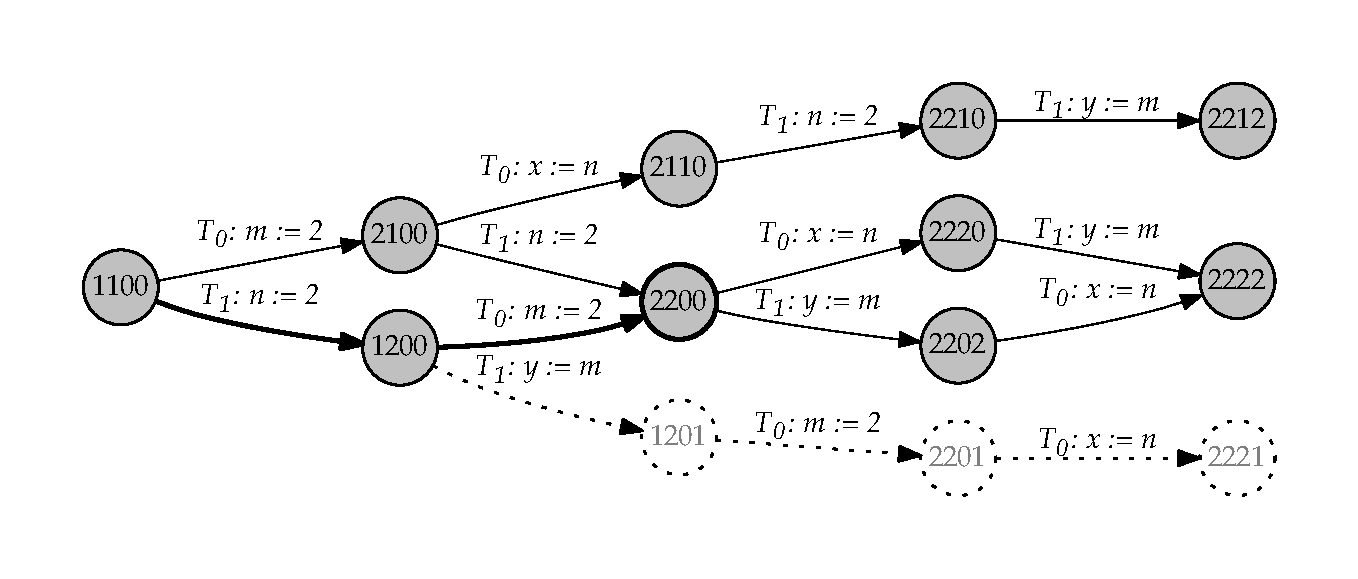
\includegraphics[width=\textwidth]{sdpor}
	\end{subfigure}
	\caption[An example illustrating the need for the
		Stateful DPOR algorithm.]
		{An example showing that na\"{\i}vely
		cutting short the DPOR algorithm is
		unsound. Each state in the diagram shows
	the values of \textit{mnxy}.}
	\label{fig:sdpor-motivation}
\end{figure}

\subsubsection{Stateful Dynamic Partial-Order Reduction}

One such method is to use a \emph{visible operation dependency
graph}, proposed by Yang et al.\@ in an
algorithm known as stateful dynamic
partial-order reduction (SDPOR) \cite{yang08}.
The idea is that when we first explore
a section of the state space,
we make a note of the visible operations
that may be executed, so that if we encounter that section again,
we can cut short the search, and use our knowledge of the
visible operations that may have been
executed if the search was continued
to add backtracking points as necessary.

More precisely, a visible operation dependency
graph is a graph $G = \langle V, E \rangle$ whose
nodes represent visible operations, and whose edges
represent the ordering of those transitions; whenever
a transition sequence of the form
$\sigma_1 \xrightarrow{t} \sigma_2 \xrightarrow{t'}
 \sigma_3$
is encountered in a search of the state space, the
edge $(t, t')$ is added to the visible operation
dependency graph $G$. Then, when a state $\sigma$ is
encountered which has already been explored on the
search, sufficient backtracking points for soundness
can be added by calling the
\textsc{UpdateBacktrackSets} procedure
on each transition in the set
\[\mathcal{U} = \{u \mid \exists t \in \textit{enabled}(\sigma).\;
   u \text{ is reachable from node } t \text{ in graph } G\}.\]
For its efficiency, SDPOR relies on the assumption that
the sets $\mathcal{U}$ of reachable transitions
are generally small in size.

The pseudocode for the SDPOR algorithm is shown
in Appendix~\ref{sapp:sdpor-code}.
To implement the visible operation dependency graph
$G$, I chose to use another hash table,
mapping from transitions to lists of transitions.
Calling \textsc{UpdateBacktrackSets} on
each reachable node in $G$ is implemented using
a simple depth-first search.

\subsection{Static Partial-Order Reduction}
\label{sec:spor-imp}

In order to evaluate the improvement in performance
allowed by building persistent sets dynamically
instead of statically, I decided to research and
implement a static partial-order reduction
(SPOR\footnote{Not to be confused with SDPOR.})
algorithm. However, I struggled to find one
in the literature that I could
understand and implement in the available time.
I therefore designed my own
rudimentary static persistent-set algorithm, which,
while easy to understand and implement,
usually returns unfortunately large persistent sets.

Before the algorithm begins its search, it compiles a table
listing all the shared objects that each process may
access, then, during the search, persistent sets $T$ are
constructed such that
every process whose next transition is
not in $T$ never accesses any
object that any process whose next
transition is in $T$ accesses.
The pseudocode for this procedure is
given in Appendix~\ref{sapp:spor-code}.
While it may seem that computing
the objects the threads can access
should be done at every state rather than
just once, this is actually prohibitively
expensive and offers only modest
reductions in the sizes of the
persistent sets.

A limitation of my algorithm is that
it assumes that each threads accesses
only shared objects
explicitly mentioned in its own
local state so using shared objects
to communicate references to other shared
objects may result in unsound persistent
sets being chosen.

\subsection{Sleep Sets}

To implement sleep sets, as
explained in Section~\ref{sec:sleep-prep},
I adapted my
code for the simple model-checking
algorithm to match the pseudocode
given in Appendix~\ref{sapp:sleep-code}.
As usual, I used a
library hash table implementation,
and used lists of process identifiers
to represent sleep sets, since one
integer takes up less memory
than one representation of a transition,
while providing sufficient information
for this purpose.

Applying the sleep-set technique to the
dynamic partial-order reduction
algorithm involves keeping track of the
sleep sets in the same way, and never
adding backtracking points for
processes that are in the sleep set
of the relevant state. This is
sound, although not as obviously as
it might first seem \cite[Theorem~1]{flan05addm}.

\chapter{Evaluation}
\label{cha:evaluation}

After reading this chapter,
you should understand:
\begin{understandinglist}
	\item the extent to which I believe
	my implementations are correct, and the evidence
	motivating that belief;
	\item why being certain of the
	soundness of a model-checking
	system is not essential for it
	to be of practical use; and
	\item how the model-checking
	algorithms I implemented perform
	in relation to one another.
\end{understandinglist}

\section{Soundness}

Although the various model-checking algorithms
have all been proven sound, bugs in my
project could easily render my implementations
of them incorrect.
After reading this section, you should understand
the extent to which I believe
my implementations are correct and why, and how
verification systems can be useful despite
not being verified themselves.

\subsection{Evidence for Soundness}
Almost every program contains bugs---industry average
is about 1 to 25 errors per 1,000 lines
of delivered code \cite{mccon04}.
My project consists of
at least 3,250 lines of code,
and there is no reason to think that I would
produce fewer errors than the average
professional software developer, so
it is likely it contains several defects.
However, I believe that
all remaining bugs in my project
probably relate
to functionality not necessary for
soundness. For instance, I would
not be surprised if there were a bug
in my implementation of PL,
whereas I would not expect
my implementation of DPOR to
return an incorrect result.
There are two main reasons
for this belief: my review and understanding
of the code, and my testing process.

\subsubsection{Review of Source Code}
OCaml is high-level enough that 
side-by-side comparison of my code
and the corresponding pseudocode reveals
the mapping of one onto the other. This
makes it relatively easy to perform
thought experiments to try to find
differences in semantics between the two.
During development, I spent time doing this,
successfully discovering some bugs; at
the end of the process, I am more
confident in the correctness of my implementations
as a result---especially
the simple model checker,
due to its simplicity.

\subsubsection{Tests}
\label{sec:pl-checker-tests}
As part of the development process,
I wrote 45 varied test cases, each
consisting of a PL program and
the expected
$(\textit{error-free},\, \textit{deadlock-free})$
result of model checking that transition
system.
Running a
model-checking algorithm on the
program should give the expected
result. If not, then either
I expected the wrong result,
or the implementation was incorrect.
Because of my confidence in its
correctness, I used the simple
model checker to verify
my expectations, so that any
unexpected result implied the
existence of a bug.

Although the tests were primarily designed
to help me find bugs during
development, they have the
secondary benefit of increasing the
confidence in my implementations---only
obscure bugs could
elude my tests, assuming that the
code coverage is as good as I think.

\subsection{Model Checking In Practice}
Verification of my implementations
would take months of
effort, and is significantly out
of the scope of my project.
Although it may initially seem
that a model-checking system without
such a guarantee of its
soundness is useless, this
is not the case.

It can be argued \cite{demi79}
that proof of a statement
is best understood as a social process
by which a consensus arises in its
truth, and that formal proofs are a relatively
poor catalyst to this process, since
they are so long and difficult to
read.
There are other
ways that the confidence in a program's
correctness can be increased, including
conventional testing, successful
long-term use, and performing
cross-checking with other (ideally
independently developed) implementations
\cite{beck06, tau02}.

In practice, factors such as
performance and usability are at least
as important as soundness. A system that
catches 90\% of bugs can still be a
useful tool, especially if it catches
errors which are difficult to expose
using conventional testing, such as
those caused by race conditions. 
Conversely, if a system
is guaranteed to be sound, but takes an
impractically long time to check any realistic
program, or if it requires
weeks of training before use,
then it will not be used in
practice.
Similarly, a system that
returns only a single Boolean result
is less useful
than one like my project, which points the developer
in the direction of the bug if
one is found.

Perhaps the clearest indication of the
value of unverified
model-checking systems is their widespread
industrial use and resulting successes.
\cite{kur08, brat04, low96, kars96, cof10, mill08, new15}
It is also noteworthy that, as of 2006,
there were only
two verified model-checking
systems despite model
checking having been in use for
over two decades,
neither of which was widely
used \cite{beck06}.


\section{Performance}
After reading this section, you should
understand how effective the different
model-checking algorithms are at
addressing the state explosion
problem, and how efficient
my implementations of them are.

\subsection{Methodology}
Unfortunately, there is no concurrent program
that is ``typical'' for verification by model
checking. I have therefore had to pick some
example programs for which to analyse the performance
of the algorithms. For each of these examples, I varied
some test parameter and recorded for each algorithm
both the number of (not necessarily unique) transitions
explored, which is a measure of how successful
the algorithm is in addressing the state
explosion problem, and also
the execution time, which is what ultimately
matters in practice.

The examples
I chose (explained below) feature a lot
of interaction between threads relative
to many real-world programs, in which
each thread will often perform a lot
of work without interacting with any
other threads. This means that the
algorithms, particularly DPOR, are likely to be more
effective on such programs.

The numbers of transitions explored were easily
obtained by counting the numbers of recursive calls made.
The execution times were measured using the \texttt{time}
function in the Sys module packaged with OCaml. It returns
measurements of time only in quanta of 0.004 seconds,
so the accuracy of the time measurements is poor for
executions not much longer than this time.
The precision of measurements
is good, though, with very similar results being returned
for multiple executions of the same program.
Having established this,
I took only one measurement
for each, preferring
to focus effort on collecting data
from more examples.

\subsubsection{Example 1 -- Repeated Accesses}
Each thread in this example is assigned a particular
shared object, which it accesses a
fixed number of times. There are three test parameters:
the total number of threads, the number of threads
assigned to each shared object, and the
number of accesses that each thread
makes. This example allows
the amount of dependence between the threads
to be controlled by varying this second parameter.
\newpage
\subsubsection{Example 2 -- Bounded Buffer}
This is an instance of Dijksta's classic bounded-buffer problem
\cite{dijk74},
in which two threads operate on a shared fixed-length
array of items, with the ``producer''
writing new items to the buffer and the
``consumer'' removing them.
I used a buffer of size 8 and effected mutual
exclusion using per-item locks. By varying
the number of items that each thread processes
as the test variable, this example explores
how the algorithms perform as the number
of instructions per thread increases on a
more realistic example.

\subsubsection{Example 3 -- Indexer}
Taken from the paper introducing DPOR
\cite[Figure~1]{flan05}, each
thread ``receives'' a number of
``messages'', each of which is inserted
into a shared hash table. If a slot
is already occupied, the
next free slot is tried instead.
This example was chosen to allow
comparison with the published
results \cite[Figure~8]{flan05}, and to evaluate the algorithms
on a realistic use case.

\subsubsection{Example 4 -- File System}
Also from the DPOR paper
\cite[Figure~7]{flan05}, this example is
based an idiom found in the Frangipani file
system \cite{thek97}.
Each thread searches for a free
``disk block'' for an ``inode'' to point
to. This example was chosen for
the same reasons as Example 3.

\subsection{Results}
For each example program, the results for all eight
algorithms are presented on the same graph, in the
style indicated in Figure~\ref{fig:key}.
If the timing function
returned 0.000s, I plotted a point at 0.002s
for clarity, since
$\log(0)$ is undefined.
I stopped collecting data when execution
times approached 100 seconds.

\begin{figure}[h]
	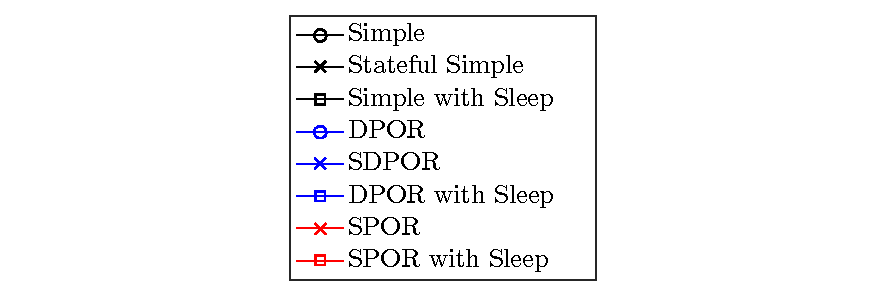
\includegraphics[width=\textwidth]{key}
	\caption{Key for model-checking algorithm performance graphs.}
	\label{fig:key}
\end{figure}

\begin{figure}
	\centering
	\footnotesize
	\begin{figtile}
		\input{figs/t43_tpl1_ops1.pdf_tex}
		\caption{1 thread per object,
			each making 1 access.}
	\end{figtile}%
	\quad
	\begin{figtile}
		\input{figs/t43_tpl1_ops3.pdf_tex}
		\caption{1 thread per object,
			each making 3 accesses.}
	\end{figtile}
	\begin{figtile}
		\input{figs/t43_tpl2_ops1.pdf_tex}
		\caption{2 threads per object,
			each making 1 access.}
	\end{figtile}%
	\quad
	\begin{figtile}
		\input{figs/t43_tpl2_ops3.pdf_tex}
		\caption{2 threads per object,
			each making 3 accesses.}
	\end{figtile}
	\begin{figtile}
		\input{figs/t43_tpl3_ops1.pdf_tex}
		\caption{3 threads per object,
			each making 1 access.}
	\end{figtile}%
	\quad
	\begin{figtile}
		\input{figs/t43_tpl3_ops3.pdf_tex}
		\caption{3 threads per object,
			each making 3 accesses.}
	\end{figtile}
	\begin{figtile}
		\input{figs/t43_tpl4_ops1.pdf_tex}
		\caption{4 threads per object,
			each making 1 access.}
	\end{figtile}%
	\quad
	\begin{figtile}
		\input{figs/t43_tpl4_ops3.pdf_tex}
		\caption{4 threads per object,
			each making 3 accesses.}
		\label{fig:repeated-access-trans-h}
	\end{figtile}
	\caption{Numbers of transitions
		explored for the repeated-accesses example.}
	\label{fig:repeated-access-trans}
\end{figure}

\begin{figure}
	\centering
	\footnotesize
	\begin{figtile}
		\input{figs/t43_time_tpl1_ops1.pdf_tex}
		\caption{1 thread per object,
			each making 1 access.}
	\end{figtile}%
	\quad
	\begin{figtile}
		\input{figs/t43_time_tpl1_ops3.pdf_tex}
		\caption{1 thread per object,
			each making 3 accesses.}
	\end{figtile}
	\begin{figtile}
		\input{figs/t43_time_tpl2_ops1.pdf_tex}
		\caption{2 threads per object,
			each making 1 access.}
	\end{figtile}%
	\quad
	\begin{figtile}
		\input{figs/t43_time_tpl2_ops3.pdf_tex}
		\caption{2 threads per object,
			each making 3 accesses.}
	\end{figtile}
	\begin{figtile}
		\input{figs/t43_time_tpl3_ops1.pdf_tex}
		\caption{3 threads per object,
			each making 1 access.}
	\end{figtile}%
	\quad
	\begin{figtile}
		\input{figs/t43_time_tpl3_ops3.pdf_tex}
		\caption{3 threads per object,
			each making 3 accesses.}
	\end{figtile}
	\begin{figtile}
		\input{figs/t43_time_tpl4_ops1.pdf_tex}
		\caption{4 threads per object,
			each making 1 access.}
	\end{figtile}%
	\quad
	\begin{figtile}
		\input{figs/t43_time_tpl4_ops3.pdf_tex}
		\caption{4 threads per object,
			each making 3 accesses.}
		\label{fig:repeated-access-time-h}
	\end{figtile}
	\caption{Execution times for the repeated-accesses example.}
	\label{fig:repeated-access-time}
\end{figure}

\begin{figure}
	\centering

	\def\svgwidth{\textwidth}
	\input{figs/prod_cons_trans_fig.pdf_tex}
	\caption{Numbers of transitions explored
		for the bounded-buffer example.}
	\label{fig:prod-cons-trans}
	\def\svgwidth{\textwidth}
	\input{figs/prod_cons_time_fig.pdf_tex}
	\caption{Execution times for the
		bounded-buffer example.}
	\label{fig:prod-cons-time}
\end{figure}

\begin{figure}
	\centering

	\def\svgwidth{\textwidth}
	\input{figs/indexer_trans_fig.pdf_tex}
	\caption{Numbers of transitions explored
		for the indexer example.}
	\label{fig:indexer-trans}

	\def\svgwidth{\textwidth}
	\input{figs/indexer_time_fig.pdf_tex}
	\caption{Execution times
		for the indexer example.}
	\label{fig:indexer-time}
\end{figure}

\begin{figure}
	\def\svgwidth{\textwidth}
	\input{figs/fs_trans_fig.pdf_tex}
	\caption{Numbers of transitions explored
		for the file-system example.}
	\label{fig:fs-trans}

	\def\svgwidth{\textwidth}
	\input{figs/fs_time_fig.pdf_tex}
	\caption{Execution times
		for the file-system example.}
	\label{fig:fs-time}
\end{figure}

\newpage
\subsection{Performance of the Algorithms}

\subsubsection{Simple Model Checker}
The simple model checker provides a
baseline, exploring every path from
the initial state to a stopped state
exactly once. Due to the state explosion
problem, this number increases
exponentially with the complexity
of the program being verified.
As constant work is done per thread per transition
explored, the execution times of the simple
algorithm are
proportional to the number of transitions it
explores.

\subsubsection{Stateful Simple Model Checking}
The stateful simple model-checker can be
seen to perform consistently well, in terms
of reduction of the explored state space.
If two transitions are ``actually'' independent,
meaning that executing them in either order
results in the same state, then the stateful
algorithm should explore from only one of these;
the prevalence of such pairs of transitions
explains the success of this approach.

Despite the reductions in the numbers
of transitions explored, the cost of
the hash-table operations
necessary for stateful checking means that
the execution times
are sometimes worse than for the
simple algorithm---for example,
in Figure~\ref{fig:indexer-time}.
However, looking at Figure~\ref{fig:repeated-access-time}
suggests that this is only a short-term
problem, and as the size of the state
space increases, the benefits of
stateful model checking
dominate its costs.

\subsubsection{Dynamic Partial-Order Reduction}
When all transitions are independent,
as in the first two cases of
Figure~\ref{fig:repeated-access-trans},
the DPOR algorithm only explores
one execution path, with negligible cost.
In the other cases in
Figure~\ref{fig:repeated-access-trans},
adding an extra thread is either of
negligible cost (if and only if the new thread
is independent of the others), or
contributes a multiplicative
increase to the cost of the search.
These multiplicative increases are
still not as severe as in the
simple algorithm, though, because the new
thread is independent of at least some of
the existing threads.

In the bounded-buffer example
(Figure~\ref{fig:prod-cons-trans}),
the DPOR algorithm is able to exploit
the independence between the two threads
(they are dependent only when they
access the same item in the buffer) to
slow the
exponential cost caused by the
state explosion problem.

The remaining two examples are more
realistic in nature, and exemplify the
benefits that DPOR can offer.
In the indexer example
(Figure~\ref{fig:indexer-trans}),
dependence between
threads is caused only by collisions
in the hash table---for the simple
hash function used, this happens at twelve threads,
but for realistic hash functions would
happen much later. Since there are no
race conditions if there are no collisions,
only one execution path
is explored for fewer than twelve threads.
Similar behaviour is seen in
Figure~\ref{fig:fs-trans}, in which only
one path is explored until similar ``collisions''
when accessing a table occur.

Theoretically, DPOR does a fixed amount of
work per thread per transition, including some
memory operations to keep track of the backtrack
sets. As the number of transitions explored
varies with
the number of threads much more than the amount
of work per transition explored does, I would
expect the execution times to be roughly
proportional to the numbers of transitions
explored. Incidentally, the fact that this is consistently
the case, and that the graphs of transitions
explored match their published counterparts
\cite{flan05},
is further evidence that my
implementation is correct and not
unnecessarily complex.

\subsubsection{Stateful Dynamic Partial-Order Reduction}
In the cases given above, the SDPOR algorithm
consistently performs poorly, exploring at
least as many transitions as the plain
DPOR algorithm. However, in the examples
given by Yang et al.\@ \cite{yang08},
SDPOR consistently performs better.
The explanation for this seems to be that
their examples are much larger, meaning
that when a state is re-encountered,
a larger saving is typically made,
while the number of backtracking
points introduced does not increase
in the same way. It would be interesting
to investigate exactly when the SDPOR
algorithm outperforms stateless DPOR.

However, as seen in Figures
\ref{fig:indexer-time} and \ref{fig:fs-time},
the execution times for the SDPOR algorithm
are much worse than what might be
expected given the number of
transitions it explores.
This can be explained by the increasing
costs of the hash-table operations
performed at each state, since each
state occupies quite a lot of memory.

As well as introducing SDPOR, Yang et al.\@
also introduced a light-weight
scheme for capturing the local states of
threads, which they used in conjunction with
SDPOR to improve its implementation efficiency.
Had I implemented this additional
technique, the average cost of the hash-table
operations would have decreased, although
the large numbers of transitions explored
would not have been affected.

\subsubsection{Sleep Sets}
For the simple model-checker,
sleep sets significantly reduce the
rate of exponential increase in
the number of transitions explored in every example,
by preventing the
unnecessary re-exploration of sections
of the state space (more effectively
than the simple stateful algorithm).

When applied to the DPOR algorithm, the results
are more variable. While little benefit is seen
from applying sleep sets to DPOR in
Figures~\ref{fig:repeated-access-time}
and \ref{fig:indexer-trans}
(presumably because the DPOR algorithm has already
fully exploited the independence between the threads),
better results are seen in 
Figures~\ref{fig:prod-cons-trans} and \ref{fig:fs-trans},
in which sleep sets work
in conjunction with DPOR to greatly
slow the rate of the exponential increase in the
number of transitions explored.
Although the effectiveness of the technique
depends on the particular program being
verified, it seems that on more realistic
examples, it is highly effective.

There is a time and space cost in
applying the sleep-set technique.
In the repeated-accesses example,
using sleep sets does not reduce the number
of explored transitions when applied
to DPOR, so this time cost can be clearly
seen in Figure~\ref{fig:repeated-access-time}.
However, in the other examples, and all
realistic programs, these
costs are insignificant compared
to the considerable benefits available.

\subsubsection{Static Partial-Order Reduction}
When every thread accesses separate objects,
then my SPOR algorithm returns persistent sets
of size one, which is optimal, as shown in the
first two cases of
Figure~\ref{fig:repeated-access-trans}.
However, this is very much a corner case,
and my SPOR algorithm usually offers only
modest reductions in the number of transitions
explored---as the number of threads sharing
each object increase, the benefits of the
algorithm decrease.

In particular, if the threads of
a program cannot be partitioned
such that the objects accessed by different
partitions are disjoint, my SPOR algorithm
offers no improvements at all. Unfortunately, this
is the case for most concurrent programs,
including my other examples, from which
the SPOR results have therefore been omitted.

The extra work done per transition
in implementing my SPOR
algorithm is by design little
(cf. Section~\ref{sec:spor-imp}), so
execution times are roughly proportional
to the number of transitions explored.

Once again, attempting to implement
an SPOR algorithm mostly served to give
me a greater understanding
of the difficulty of trying to
statically compute reasonably small persistent sets.

\chapter{Conclusions}

\section{Summary and Reflections}

As well as meeting the aims of the
project, I also
managed to implement several
extensions, allowing a fuller
analysis of the benefits of
DPOR in relation to other
related techniques.
The performance
of the implemented algorithms
was quantitatively evaluated,
revealing that DPOR is often
very effective at mitigating
the state explosion problem,
especially when used in
conjunction with the
sleep-set technique.

Despite the considerable
challenges, particularly in
understanding
the model-checking algorithms
and their underlying theory, the
satisfaction of eventually achieving
my goals was gratifying. Besides
being a subject that I am interested
in, I am glad that I chose this project because
it has allowed me to develop the important skills
of reading academic papers, translating high-level
algorithms into executable programs, and
developing software.


\section{Further Work}
Instead of assuming that any
two processes that access the
same object must be dependent,
it is possible to distinguish
between reads and writes to
shared objects, allowing
two consecutive reads to be identified
as independent (in the sense of
Section~\ref{sec:independence}).
Flanagan and Godefroid suggest
that this could be implemented
by keeping two clock vectors per
shared object---one for reads and
the other for writes \cite{flan05}.
It would
be interesting to implement
this algorithm and evaluate its
performance in relation to the
original DPOR algorithm.

I would also like
to use my system to verify
programs written in a widely-used
language; as mentioned previously,
the only work necessary for this
is an implementation of the
\textit{Expression} and
\textit{Thread} modules.
Given the complexity of some modern
programming languages, though,
this might not be trivial. A better
approach for Java, for example,
might be to implement a JVM which
performs DPOR, inspired by
Java PathFinder \cite{viss03}.

Finally, I would be
be interested in spending time
looking at recent developments
in model checking
that have been made since
the introduction of DPOR.

\newpage
\null
\thispagestyle{plain}

%%%%%%%%%%%%%%%%%%%%%%%%%%%%%%%%%%%%%%%%%%%%%%%%%%%%%%%%%%%%%%%%%%%%%
% the bibliography
\addcontentsline{toc}{chapter}{Bibliography}
\bibliography{refs}

%%%%%%%%%%%%%%%%%%%%%%%%%%%%%%%%%%%%%%%%%%%%%%%%%%%%%%%%%%%%%%%%%%%%%
% the appendices
\appendix
% Hide subappendices from contents
\addtocontents{toc}{\setcounter{tocdepth}{0}}

\chapter{Details of DPOR}
\vspace{-0.5cm}
\section{Explanation of Theory}
\label{app:dpor-walkthrough}
\dporpseudocode
\begin{description}
	\item[Lines 1--2] The \textsc{Explore} procedure implements
	dynamic partial-order reduction. The transition sequence
	$\pi$ which is passed as its argument implicitly specifies the state
	from which the exploration is to take place, $\sigma$.

	\item[Lines 3--4] First, any necessary backtracking points
	which can be identified from this state are added to the
	\textit{backtrack} sets of previous states. Backtracking
	points can be identified using information from each possible
	transition from this state, so the \textsc{UpdateBacktrackSets}
	procedure is called with each possible next transition as an
	argument.

	\item[Line 5] Having updated the \textit{backtrack} sets
	of previous states, the search continues its exploration,
	but only if there are any enabled transitions to explore.

	\item[Lines 6--8] The recursive exploration proceeds by
	maintaining two sets of transitions: \textit{backtrack}
	and \textit{done}. The \textit{backtrack} set contains
	those transitions from $\sigma$ which should be explored,
	and is initialised to contained any single enabled transition.
	Recursive calls to
	\textsc{Explore} may add more transitions to \textit{backtrack}.
	The \textit{done} set contains those transitions
	in \textit{backtrack} that have been explored.

	\item[Line 9] The search from $\sigma$ halts when every
	transition that needs to be explored (is in \textit{backtrack})
	has been explored (is in \textit{done}).

	\item[Lines 10--12] If there is some transition that needs
	exploring, \textsc{Explore} is recursively called with that
	transition extending the current transition sequence $\pi$,
	and that transition is added to \textit{done}.

	\item[Line 14] The \textsc{UpdateBacktrackSets} procedure
	can use the information that a given transition, $t_{p,s}$ can be
	executed in $\sigma$ to add necessary backtracking points.

	\item[Line 15] The set $D$ contains the indices $i$ of the
	transitions $\pi_i$ in the sequence such that $\pi_i$ and
	$t$ are dependent, and $(i, p)\!\not \hookrightarrow_\pi$.
	This second condition means that $t_{p,s}$ is \emph{not}
	guaranteed to happen after $\pi_i$, so $D$ is the set
	of transitions which may have a race condition with
	$t_{p,s}$.

	\item[Line 16] If there are no transitions which have
	a race condition with $t_{p,s}$, then no backtracking
	points need to be added: as far as we know from $t_{p,s}$,
	if we had chosen any other
	choices of transitions to explore previously, we would
	have ended up with a transition sequence in the same
	equivalence class as $\pi$.

	\item[Line 17] If there are transitions in $\pi$
	which have a race condition with $t_{p,s}$, then
	it is sufficient to add a backtracking point at
	the state immediately before
	the most recent of these;
	the necessary backtracking
	points for the earlier states will be added
	by later (or previous) calls of \textsc{Explore}.

	\item[Line 18] We know there is a race condition
	between $t_{p,s}$ and $\textit{next}(\sigma_d,p)$, so
	we want to explore another transition sequence from
	$\sigma_d$ in which $\textit{next}(\sigma_d,p)$
	appears before $t_{p,s}$. If $\textit{next}(\sigma_d,p)$
	is enabled in $\sigma_d$, then we certainly explore such
	a transition sequence by immediately exploring
	$\textit{next}(\sigma_d,p)$ from $\sigma_d$.

	\item[Line 19] However, if we cannot immediately
	explore $\textit{next}(\sigma_d,p)$
	from $\sigma_d$ because it is not enabled, then it is
	not obvious which transitions to explore from $\sigma_d$
	to achieve
	a transition sequence in which $\textit{next}(\sigma_d,p)$
	appears before $t_{p,s}$. The algorithm presented here
	does not attempt to narrow down which transitions might
	lead to such a transition sequence, and instead plays it
	safe and explores them all.

	\item[Lines 21] To perform model checking, the state space
	is explored from the initial state, $\sigma_0$, which is
	reached from $\sigma_0$ by executing no transitions, so
	\textsc{Explore} is initially called on the empty
	sequence of transitions, $\emptyset$.

\end{description}

\section{OCaml Implementation}
\label{sapp:dpor-imp}
Below is my OCaml implementation of the DPOR
algorithm. Note that many of the comments are
references to the original pseudocode
\cite[Figures~3--5]{flan05}, rather than the
pseudocode in this dissertation, which is
simplified for ease of understanding.

\lstinputlisting[firstline=57, lastline=188]
{../src/plain_checker.ml}

\chapter{Other Model-Checking Algorithms}
\label{app:pseudocode}
\section{Simple Model Checker}
\label{sapp:simple-code}
\begin{algorithmic}[1]
	\Procedure{Check}{$\sigma_0,\,\pi$}
	\Let{$(l, g)$}
	{$\textit{last}(\pi)$}
	\Let{\textit{error\_free}}{true}
	\Let{\textit{is\_enabled\_thread}}{false}
	\Let{\textit{no\_waiting\_threads}}{true}
	\Let{\textit{calls\_deadlock\_free}}{true}
	\ForAll{$p \in \mathcal{P}$}
	\If{$\textit{next}(\sigma, p) \in \textit{enabled}(\sigma)$}
	\State \textit{is\_enabled\_thread} := true;
	\Let{$(\textit{result\_ef}, \textit{result\_df})$}
	{\Call{Check}{$\sigma_0, \pi.\textit{next}(\sigma, p)$}}
	\State \textit{error\_free} := \textit{error\_free}
	\& \textit{result\_ef};
	\State \textit{calls\_deadlock\_free}
	:= \textit{calls\_deadlock\_free}
	\& \textit{result\_df}
	\Else
	\If{$\textit{err}(l(p))$}{ \textit{error\_free} := false};
	\EndIf
	\If{$\exists g' \in \mathcal{G}.\;
		\textit{next}(\sigma,p) \in \textit{enabled}(l,g')$}
	{\textit{no\_waiting\_threads} := false}
	\EndIf
	\EndIf
	\EndFor
	\Let{\textit{deadlock\_free}}{\textit{calls\_deadlock\_free} \&
		(\textit{is\_enabled\_thread} | \textit{no\_waiting\_threads})}
	\State \Return (\textit{error\_free}, \textit{deadlock\_free})
	\EndProcedure
\end{algorithmic}

The algorithm assumes that if a thread
encounters an error, then the execution
of that thread will not proceed, meaning
that only threads which do not have any
enabled transitions need to be checked
for errors. The Boolean \textit{error\_free}
is set to false if an error is encountered
either in this state (line 14) or in a
recursive call (line 11).

Deciding whether the state space from the current
state onwards is deadlock-free is more complicated.
The \textit{calls\_deadlock\_free} keeps track of
whether any recursive call reports a deadlock (line 12).
The current state is not a deadlock state
if either there is some thread with an
enabled transition,
or every thread had terminated its computation and
is not waiting for some change in the shared state.
If any transition is enabled, then
\textit{is\_enabled\_thread} is set to true (line 9).
If any thread without an enabled transition is
waiting for some change in the shared state (for
instance a lock to become available), then
\textit{no\_waiting\_threads} is set to false.
These results are combined in line 17.

\section{Stateful Dynamic Partial-Order Reduction}
\label{sapp:sdpor-code}
\begin{algorithmic}[1]
	\Let{$H$}{an empty hash table of states}
	\Let{$G$}{an empty graph on transitions}
	\State
	\Procedure{Explore}{$\pi$}
	\Let{$\sigma$}{$\textit{last}(\pi)$}
	\If{$\sigma \in H$}
	\Let{$\mathcal{U}$}
	{$\{u \mid \exists t \in \textit{enabled}(\sigma).\;
		u \text{ is reachable from node }
		t \text{ in } G\}$}
	\ForAll{$t \in \mathcal{U}$}
	\Call{UpdateBacktrackSets}
	{$\pi,\, t$}
	\EndFor
	\Else{
		\State add $\sigma$ into $H$;
		\ForAll{$p \in \mathcal{P}$}
		\Call{UpdateBacktrackSets}
		{$\pi,\, \textit{next}(\sigma, p)$};
		\EndFor
		\If{$\textit{enabled}(\sigma) \neq \emptyset$}
		\Let{$t$}{any $t \in \textit{enabled}(\sigma)$}
		\Let{$\textit{backtrack}(\sigma)$}{$\{t\}$}
		\Let{$\textit{done}(\sigma)$}{$\emptyset$}
		\While{$\textit{done}(\sigma)
			\neq \textit{backtrack}(\sigma)$}
		\Let{$t$}{any $t \in (\textit{backtrack}(\sigma)
			\setminus \textit{done}(\sigma))$}
		\State add $t$ to $\textit{done}(\sigma)$;
		\If{$|\pi| > 0$}
		add edge $(\pi_{|\pi|-1}, t)$ to $G$;
		\EndIf
		\State \Call{Explore}{$\pi.t$}
		\EndWhile
		\EndIf
	}\EndIf
	\EndProcedure
	\State
	\Procedure{UpdateBacktrackSets}{$\pi,\, t_{p,s}$}
	\Let{$D$}{$\{i \in \textit{dom}(\pi) \mid
		\pi_i \text{ is dependent with } t_{p,s}
		\text{ and } i \not \hookrightarrow_\pi p\}$}
	\If{$D \neq \emptyset$}
	\Let{$\sigma_d$}
	{$\textit{pre}(\pi,\text{max}(D))$}
	\If{$\textit{next}(\sigma_d, p)
		\in \textit{enabled}(\sigma_d)$}
	add $\textit{next}(\sigma_d, p)$
	to $\textit{backtrack}(\sigma_d)$
	\Else {
		add all of $\textit{enabled}(\sigma_d)$
		to $\textit{backtrack}(\sigma_d)$
	} \EndIf
	\EndIf
	\EndProcedure
	\State
	\State Initially: \Call{Explore}{$\emptyset$}
\end{algorithmic}
\newpage
\section{Static Partial-Order Reduction}
\label{sapp:spor-code}
\begin{algorithmic}[1]
	\Procedure{PersistentSet}{$\sigma$}
	\Let{$E$}{$\{p\}$,
		for any $p$ such that
		$\exists t_{p,s} \in \textit{enabled}(\sigma)$}
	\Let{$O$}{$\{o \mid \textit{accesses}(p, o)\}$}
	\While{$E$ changes}
	\ForAll{$q \in (\mathcal{P} \setminus E)$}
	\If{$\exists o \in O.\;
		\textit{accesses}(q,o)$}
	\State $E := E \cup \{p\}$;
	\State $O := O \cup \{o \mid
	\textit{accesses}(q, o)\}$
	\EndIf
	\EndFor
	\EndWhile
	\Let{$T$}{$\{t \mid \exists p \in E.\;
		t = \textit{next}(\sigma,p)\}$}
	\If{$(T \setminus \textit{enabled}(\sigma))
		\neq \emptyset$}
	\Return $\textit{enabled}(\sigma)$
	\Else \ \Return $T$
	\EndIf
	\EndProcedure
\end{algorithmic}
\vspace{1.5cm}
\section{Sleep Sets}
\label{sapp:sleep-code}

This pseudocode is adapted from pseudocode
given by Godefroid \cite{god96}, the main
difference being that Godefroid uses
iteration and an explicit stack, rather
than recursion.
\smallskip
\begin{algorithmic}[1]
	\Let{$H$}{an empty hash table mapping
		states to sets of transitions}
	\State
	\Procedure{Check}{$\sigma,\, \textit{Sleep}$}
	\If{$\sigma \not \in H$}
	\State add $(\sigma, \textit{Sleep})$ to $H$;
	\State$T := \textit{enabled}(\sigma)
	\setminus \textit{Sleep}$
	\Else
	\State$T := H(\sigma) \setminus
	\textit{Sleep}$;
	\State $\textit{Sleep} := \textit{Sleep}
	\cap H(\sigma)$;
	\State $H(\sigma) := \textit{Sleep}$
	\EndIf
	\ForAll{$t \in T$}
	\Let{$\sigma'$}{$\sigma'$ such that
		$\sigma \xrightarrow{t} \sigma'$}
	\Let{$\textit{Sleep}'$}{$\{t' \in \textit{Sleep}
		\mid t' \text{ is independent with } t\}$}
	\State\Call{Check}{$\sigma',\, \textit{Sleep}'$};
	\State $\textit{Sleep} := \textit{Sleep} \cup \{t\}$
	\EndFor
	\EndProcedure
	\State
	\State Initially: \Call{Check}{$\sigma_0,\, \emptyset$}
\end{algorithmic}

\chapter{Project Proposal}

\input{proposal_without_title}
\enlargethispage{1\baselineskip}

\end{document}
